\documentclass[14pt,a4paper]{extarticle}

\usepackage{iftex}
\ifPDFTeX
  \usepackage[T2A]{fontenc}
  \usepackage[utf8]{inputenc}
  \usepackage[russian]{babel}
  \usepackage{newtxtext}
\else
  \usepackage{fontspec}
  \usepackage{polyglossia}
  \setmainlanguage{russian}
  \IfFontExistsTF{Times New Roman}{%
    \newcommand{\DiplomaFont}{Times New Roman}%
  }{%
    \newcommand{\DiplomaFont}{FreeSerif}%
  }
  \setmainfont{\DiplomaFont}
  \setsansfont{\DiplomaFont}
  \setmonofont{\DiplomaFont}
  \newfontfamily\cyrillicfont{\DiplomaFont}
  \newfontfamily\cyrillicfontsf{\DiplomaFont}
  \newfontfamily\cyrillicfonttt{\DiplomaFont}
\fi

\usepackage[a4paper,left=30mm,right=10mm,top=20mm,bottom=20mm]{geometry}
\usepackage{setspace}
\onehalfspacing
\usepackage{indentfirst}
\setlength{\parindent}{1.25cm}
\setlength{\parskip}{0pt}

\usepackage{graphicx}
\usepackage{float}
\usepackage{longtable}
\usepackage{booktabs}
\usepackage{array}
\usepackage{calc}
\usepackage{multirow}
\usepackage{makecell}
\usepackage{enumitem}
\usepackage{amsmath,amssymb}
\usepackage{url}
\usepackage[hidelinks]{hyperref}

\setcounter{secnumdepth}{0}
\setcounter{tocdepth}{3}
\renewcommand{\contentsname}{СОДЕРЖАНИЕ}
\sloppy
\emergencystretch=3em
\setlist{nosep}
\renewcommand{\arraystretch}{1.2}

\providecommand{\tightlist}{%
  \setlength{\itemsep}{0pt}\setlength{\parskip}{0pt}}

\begin{document}

\tableofcontents
\clearpage

\hypertarget{ux432ux432ux435ux434ux435ux43dux438ux435}{%
\section{ВВЕДЕНИЕ}\label{ux432ux432ux435ux434ux435ux43dux438ux435}}

Цифровизация агропромышленного комплекса (АПК) является одним из стратегических приоритетов современной экономики. В рамках парадигмы «точного земледелия» беспилотные летательные аппараты (БПЛА) превратились в ключевой инструмент мониторинга посевов, аэрофотосъёмки и прецизионного внесения агрохимикатов; современные обзоры подчёркивают, что агродроны уже применяются как для дистанционного зондирования, так и для точечного внесения средств защиты растений {[}1, 2, 3{]}. По данным MarketsandMarkets, мировой рынок агро-дронов составлял около 2,63 млрд долл. США в 2025 году и прогнозируется к росту до 10,76 млрд долл. к 2030 году при среднегодовом темпе роста 32,6 \% {[}4{]}. Схожие тенденции фиксируют Fortune Business Insights: объём рынка в 2024 году оценивался в 6,10 млрд долл. при прогнозе роста до 23,78 млрд долл. к 2032 году (CAGR 18,5 \%) {[}5{]}. Российский сегмент демонстрирует ежегодный рост не менее 20 \%, что обусловлено государственными программами поддержки цифрового земледелия и уходом с рынка ряда зарубежных поставщиков агротехники.

Интеграция БПЛА в ИТ-инфраструктуру агропредприятий принципиально меняет поверхность кибератак. Беспилотный аппарат представляет собой киберфизическую систему (КФС), в которой программные уязвимости непосредственно трансформируются в физические последствия: несанкционированное управление химической нагрузкой, отклонение от маршрута или полная потеря аппарата. Исследования в области безопасности БПЛА фиксируют уязвимости на всех уровнях --- аппаратном, программном, протокольном и сенсорном {[}6, 7{]}. Особую озабоченность вызывает протокол MAVLink, де-факто являющийся стандартом связи между дроном и наземной станцией управления (НСУ): в базовой конфигурации он не обеспечивает ни шифрования данных, ни аутентификации источника сообщений {[}8{]}. Атаки на навигационные подсистемы --- GPS/ГЛОНАСС-глушение и спуфинг --- получили значительное распространение в академических исследованиях и реальных инцидентах {[}9{]}.

Актуальность темы усиливается ужесточением требований регуляторов в области информационной безопасности. Указ Президента Российской Федерации от 01.05.2022 № 250 {[}10{]} возложил персональную ответственность руководителей организаций за состояние защиты информации, а Указ Президента Российской Федерации от 30.03.2022 № 166 {[}11{]} закрепил курс на технологическую независимость и безопасность значимых объектов критической информационной инфраструктуры. ФСТЭК России в «Методике оценки угроз безопасности информации» (2021 г.) {[}12{]} установила единую обязательную методологию построения моделей угроз для государственных и критически важных информационных систем. Агропредприятия, выполняющие химическую обработку угодий с применением БПЛА, фактически управляют потенциально опасным технологическим объектом, что ставит вопрос об их соответствии требованиям к защите АСУ ТП.

Существующие коммерческие платформы управления агро-БПЛА --- DJI FlightHub 2, DroneDeploy, Pix4Dfields --- не решают задачу планирования маршрутов с учётом динамически изменяющейся киберугрозовой обстановки. Современные обзоры по БПЛА в точном земледелии подробно рассматривают сенсоры, связь, ИИ и энергоэффективность, но не закрывают прикладной сценарий автоматического перепланирования при появлении новой зоны радиоэлектронного подавления или потере отдельного дрона {[}3{]}. Таким образом, отсутствие комплексного подхода к обеспечению информационной безопасности агро-БПЛА при очевидной критичности последствий инцидентов формирует актуальную научно-практическую проблему, решению которой посвящена настоящая выпускная квалификационная работа студента (ВКРС).

Объект исследования --- информационная безопасность киберфизической инфраструктуры агропромышленного предприятия, эксплуатирующего парк беспилотных летательных аппаратов для задач точного земледелия.

Предмет исследования --- угрозы доступности и навигационной целостности БПЛА, методы их систематизации и оценки, алгоритмы безопасной маршрутизации группы БПЛА и критерии оценки надёжности миссии.

Цель работы --- разработка программной платформы автоматизированного планирования безопасных маршрутов для группы сельскохозяйственных БПЛА с учётом зон радиоэлектронного подавления, включающей модуль риск-ориентированной маршрутизации, механизм динамического перепланирования и эвристический контур обнаружения угроз по телеметрии MAVLink.

Для достижения поставленной цели решаются следующие задачи:

\begin{enumerate}
\def\labelenumi{\arabic{enumi}.}
\tightlist
\item
  Провести анализ рынка агро-дронов и обосновать целевой сегмент потребителей платформы SafeAgriRoute.
\item
  Выполнить конкурентный анализ существующих решений (DJI FlightHub 2, DroneDeploy, Pix4Dfields) и определить технологическую нишу предлагаемого продукта.
\item
  Классифицировать нарушителей и систематизировать угрозы безопасности навигации и доступности БПЛА на основе Банка данных угроз ФСТЭК России.
\item
  Формализовать метрику оценки деструктивного воздействия R(x,y) и обосновать выбор приоритетных угроз для MVP.
\item
  Спроектировать архитектуру SaaS-платформы SafeAgriRoute: модели данных, REST API, WebSocket-контур телеметрии и MAVLink-интеграцию.
\item
  Разработать алгоритм Risk-Weighted Voronoi Decomposition и CVRP-планировщик на базе Google OR-Tools с системой штрафов за пролёт через зоны РЭБ.
\item
  Реализовать алгоритм динамического перепланирования миссии при потере дрона и при появлении новой зоны РЭБ.
\item
  Провести сравнительный эксперимент и оценить эффективность предлагаемого подхода относительно базовой стратегии маршрутизации.
\end{enumerate}

Научная новизна работы состоит в следующем. Во-первых, разработана детализированная модель угроз для гетерогенных групп агро-БПЛА, включающая полный охват векторов атак на навигацию (GPS/ГЛОНАСС Jamming/Spoofing) и каналы управления (MAVLink), с привязкой к реестру БДУ ФСТЭК России. Во-вторых, предложен алгоритм Risk-Weighted Voronoi Decomposition, объединяющий пространственное разбиение зоны покрытия с риск-ориентированной балансировкой нагрузки между дронами роя. В-третьих, разработан интегральный критерий надёжности миссии (IRM), учитывающий риски всех запланированных точек маршрута, и механизм его обновления при динамическом перепланировании в режиме реального времени.

Практическая значимость определяется тем, что разработанная платформа SafeAgriRoute реализована в виде полнофункционального MVP, развёртываемого одной командой \texttt{docker-compose\ up}. Исходный код опубликован в открытом доступе по адресу \url{https://github.com/matveisut/safe-agri-route}. Система обеспечивает планирование маршрутов для поля площадью 500 га за ≤ 5 секунд и перепланирование в режиме реального времени за ≤ 500 миллисекунд для 4 дронов. Платформа протестирована посредством симуляции ArduPilot SITL и автономных Python-сценариев на модельном поле с параметрами типичного среднего агропредприятия.

Методологическую основу составляют: системный анализ, структурно-функциональное моделирование, Методика оценки угроз ФСТЭК России (2021 г.), ГОСТ Р МЭК 62443-2-1-2015, математические методы оптимизации комбинаторных задач (VRP, алгоритм Ллойда, эвристики OR-Tools), а также результаты научных публикаций из баз данных IEEE Xplore, Elsevier Computer Networks, Frontiers in Computer Science, IEEE Access, Aerospace и КиберЛенинка.

Структура работы. ВКРС состоит из введения, пяти разделов, заключения, списка использованных источников (43 наименования, из них 19 на иностранном языке). Введение обосновывает актуальность, формулирует цель, задачи и научную новизну. В разделе 1.1 проводится анализ рынка и конкурентной среды. В разделе 1.2 выполняется моделирование угроз и формализация метрики риска. В разделе 1.3 описывается архитектура платформы. В разделе 1.4 детально изложены разработанные алгоритмы. В разделе 1.5 представлены результаты экспериментальной оценки. Заключение суммирует достигнутые результаты и обозначает перспективы.


\hypertarget{ux43eux431ux449ux435ux435-ux43eux43fux438ux441ux430ux43dux438ux435-ux43fux440ux43eux435ux43aux442ux430}{%
\section{1 ОБЩЕЕ ОПИСАНИЕ ПРОЕКТА}\label{ux43eux431ux449ux435ux435-ux43eux43fux438ux441ux430ux43dux438ux435-ux43fux440ux43eux435ux43aux442ux430}}

\hypertarget{ux430ux43dux430ux43bux438ux437-ux440ux44bux43dux43aux430-ux430ux433ux440ux43e-ux434ux440ux43eux43dux43eux432-ux438-ux43aux43eux43dux43aux443ux440ux435ux43dux442ux43dux430ux44f-ux441ux440ux435ux434ux430}{%
\subsection{1.1 Анализ рынка агро-дронов и конкурентная среда}\label{ux430ux43dux430ux43bux438ux437-ux440ux44bux43dux43aux430-ux430ux433ux440ux43e-ux434ux440ux43eux43dux43eux432-ux438-ux43aux43eux43dux43aux443ux440ux435ux43dux442ux43dux430ux44f-ux441ux440ux435ux434ux430}}

\hypertarget{ux43fux440ux43eux433ux43dux43eux437-ux440ux43eux441ux442ux430-ux43cux438ux440ux43eux432ux43eux433ux43e-ux440ux44bux43dux43aux430-ux430ux433ux440ux43e-ux434ux440ux43eux43dux43eux432}{%
\subsubsection{1.1.1 Прогноз роста мирового рынка агро-дронов}\label{ux43fux440ux43eux433ux43dux43eux437-ux440ux43eux441ux442ux430-ux43cux438ux440ux43eux432ux43eux433ux43e-ux440ux44bux43dux43aux430-ux430ux433ux440ux43e-ux434ux440ux43eux43dux43eux432}}

Рынок беспилотных летательных аппаратов для агропромышленного комплекса является одним из наиболее динамично развивающихся сегментов глобальной агротехнологической индустрии. По оценке MarketsandMarkets, объём рынка агро-дронов составил около 2,63 млрд долл. США в 2025 году и при CAGR 32,6 \% достигнет 10,76 млрд долл. к 2030 году {[}4{]}. Данные Fortune Business Insights несколько расходятся по базовому году, но подтверждают общий тренд: рынок вырастет с 6,10 млрд долл. (2024 г.) до 23,78 млрд долл. к 2032 году {[}5{]}. MRFR даёт более агрессивный прогноз --- 70,58 млрд долл. к 2035 году при CAGR 24,46 \%. Столь значительный разброс оценок обусловлен различиями в методологии --- часть агентств включает в расчёт только аппаратную составляющую, другие охватывают весь стек «дрон + ПО + услуги». Тем не менее ни одна из аналитических компаний не прогнозирует CAGR ниже 18 \%, что делает рынок агро-БПЛА одним из устойчивых долгосрочных трендов в агротехе.

Таблица 1.1 --- Прогнозы мирового рынка агро-дронов от ведущих аналитических агентств



__DOCX_TABLE_MAIN_001__



Географически рынок агро-дронов концентрируется в трёх полюсах. Северная Америка занимает лидирующую позицию с долей 33,2--45 \% в зависимости от источника, опираясь на развитую нормативную базу FAA и высокий уровень государственной поддержки точного земледелия {[}4{]}. Азиатско-Тихоокеанский регион является наиболее быстрорастущим: Китай занимает первое место в мире по числу зарегистрированных агро-дронов, а компания XAG Co.~Ltd входит в топ-5 мировых производителей по объёму продаж. Европа сохраняет долю около 30 \% благодаря активному субсидированию агроинноваций в рамках программ Общей сельскохозяйственной политики ЕС. Российский сегмент, по экспертным оценкам, растёт темпом не менее 20 \% в год в условиях государственных программ импортозамещения и субсидирования закупки отечественной агротехники.

Доминирующим типом аппаратов является роторный БПЛА (мультикоптер) --- его доля в 2025 году составляла 43,7--61,7 \% в зависимости от методологии подсчёта {[}4{]}. Мультикоптеры превосходят самолётные схемы по манёвренности и способности зависать над точечными зонами обработки, что критически важно для дифференцированного внесения агрохимикатов на основе карт NDVI (Normalized Difference Vegetation Index), формируемых по результатам мультиспектральной аэрофотосъёмки. Основные сегменты применения: точное земледелие (34,7 \% выручки в 2025 г.), картографирование и мониторинг посевов, управление ирригацией.

По опубликованным оценкам, применение БПЛА снижает расход агрохимикатов на 30--40 \% по сравнению с опрыскиванием наземной техникой {[}13{]}. Практический эффект здесь связан не только с самим фактом автоматизации: дрон вносит препарат точнее, поскольку маршрут и дозировка опираются на карты NDVI и фактическое состояние посевов на отдельных участках поля. Для хозяйства это даёт ещё два прикладных преимущества: можно работать на склонах и других неудобных участках, меньше уплотнять почву тяжёлой техникой и сократить ручной труд оператора примерно на 60--70 \%.

\hypertarget{ux446ux435ux43bux435ux432ux430ux44f-ux430ux443ux434ux438ux442ux43eux440ux438ux44f-ux438-ux43fux440ux43eux444ux438ux43bux44c-ux442ux438ux43fux43eux432ux43eux433ux43e-ux43fux43eux442ux440ux435ux431ux438ux442ux435ux43bux44f}{%
\subsubsection{1.1.2 Целевая аудитория и профиль типового потребителя}\label{ux446ux435ux43bux435ux432ux430ux44f-ux430ux443ux434ux438ux442ux43eux440ux438ux44f-ux438-ux43fux440ux43eux444ux438ux43bux44c-ux442ux438ux43fux43eux432ux43eux433ux43e-ux43fux43eux442ux440ux435ux431ux438ux442ux435ux43bux44f}}

SafeAgriRoute рассчитан прежде всего на хозяйства среднего масштаба: 5 000--15 000 га и парк из 3--8 мультикоптеров грузоподъёмностью 10--20 кг. Этот диапазон выбран не формально. Крупные агрохолдинги с площадью свыше 50 000 га обычно уже содержат собственные ИТ-команды и внедряют корпоративные ERP-решения, а небольшие хозяйства до 1 000 га часто не выходят на окупаемость парка дронов: один мультикоптер-опрыскиватель стоит примерно от 900 000 до 2 500 000 рублей.

Профиль типового потребителя SafeAgriRoute включает: технического директора или главного агронома в роли лица, принимающего решение о закупке; трёх-пяти операторов БПЛА в качестве ключевых пользователей системы; ИТ-специалиста, совмещающего функции системного администратора и ответственного за информационную безопасность. Принципиально важно, что выбранный сегмент не располагает ресурсами для самостоятельной разработки и поддержки сложных ИБ-решений, что создаёт устойчивый спрос на облачные SaaS-платформы с встроенными функциями защиты.

Анализ болевых точек целевой аудитории позволяет выделить три ключевых «gap» существующих решений. Первый --- отсутствие специализированных инструментов планирования маршрутов с учётом зон радиоэлектронного воздействия (РЭБ), что критично для регионов с нестабильной радиоэлектронной обстановкой; по данным ряда экспертов, случаи кратковременного глушения сигнала ГНСС в приграничных зонах фиксируются на юге России регулярно. Второй --- невозможность автоматического перераспределения рабочей нагрузки между дронами при выходе из строя одного из аппаратов: операторы вынуждены останавливать всю миссию и перепланировать маршруты вручную. Третий --- слабое соответствие существующих зарубежных платформ требованиям ФСТЭК России и Указу № 250 {[}10{]}, что фактически исключает их использование на предприятиях, подпадающих под сферу действия этих нормативных актов.

\hypertarget{ux43aux43eux43dux43aux443ux440ux435ux43dux442ux43dux44bux439-ux430ux43dux430ux43bux438ux437-ux441ux443ux449ux435ux441ux442ux432ux443ux44eux449ux438ux445-ux43fux43bux430ux442ux444ux43eux440ux43c-ux443ux43fux440ux430ux432ux43bux435ux43dux438ux44f-ux430ux433ux440ux43e-ux431ux43fux43bux430}{%
\subsubsection{1.1.3 Конкурентный анализ существующих платформ управления агро-БПЛА}\label{ux43aux43eux43dux43aux443ux440ux435ux43dux442ux43dux44bux439-ux430ux43dux430ux43bux438ux437-ux441ux443ux449ux435ux441ux442ux432ux443ux44eux449ux438ux445-ux43fux43bux430ux442ux444ux43eux440ux43c-ux443ux43fux440ux430ux432ux43bux435ux43dux438ux44f-ux430ux433ux440ux43e-ux431ux43fux43bux430}}

Рынок программных платформ для управления агро-БПЛА к 2025 году характеризуется умеренной фрагментацией с тенденцией к консолидации {[}14{]}. Основными игроками являются DJI FlightHub 2, DroneDeploy, Pix4Dfields, Trimble AgData и ряд региональных разработчиков.

DJI FlightHub 2 --- облачная платформа управления парком дронов, нативно интегрированная с аппаратной экосистемой DJI (Agras T50, T25, Matrice 30/4). Платформа обеспечивает планирование миссий, мониторинг телеметрии в реальном времени, хранение аэрофотоданных и удалённое управление через REST API {[}14{]}. Основное ограничение --- жёсткая привязка к экосистеме DJI: аппараты других производителей (XAG, отечественный «Агромастер») интегрируются лишь частично или не поддерживаются вовсе. Функции кибербезопасности сведены к стандартным ACL и шифрованию REST-трафика; механизмы обнаружения аномалий навигации и защиты открытого канала MAVLink отсутствуют. Планирование маршрутов осуществляется по простой зональной схеме без учёта зон РЭБ.

DroneDeploy --- горизонтальная платформа, охватывающая строительство, энергетику и сельское хозяйство. В агросегменте позиционируется как инструмент создания ортофотопланов и карт NDVI с последующим формированием предписаний для дифференцированного внесения. В январе 2025 года DroneDeploy получил общенациональное разрешение на BVLOS-полёты в США {[}14{]}. Основные недостатки: высокая стоимость (корпоративные планы --- от 329 долл./мес.), отсутствие поддержки MAVLink и отсутствие ИБ-функций, специфичных для российского законодательства.

Pix4Dfields --- специализированный продукт для агрономической аналитики. Обеспечивает быструю обработку снимков непосредственно в поле (on-device), генерацию карт NDVI/NDRE и prescription maps для дифференцированного внесения. Не позиционируется как платформа управления парком: функции планирования полётных заданий ограничены, поддержки нескольких одновременно летящих дронов нет, управление миссией в реальном времени отсутствует.

Таблица 1.2 --- Конкурентное сравнение ведущих платформ управления агро-БПЛА



__DOCX_TABLE_MAIN_002__



Конкурентный анализ подтверждает наличие устойчивого технологического «gap»: ни одна из рассмотренных платформ не предоставляет функцию планирования маршрутов с учётом зон РЭБ, не реализует автоматического перепланирования при динамическом изменении обстановки и не адаптирована к российской нормативной базе в области ИБ. Именно в этом пространстве позиционируется SafeAgriRoute.

\hypertarget{swot-ux430ux43dux430ux43bux438ux437-safeagriroute}{%
\subsubsection{1.1.4 SWOT-анализ SafeAgriRoute}\label{swot-ux430ux43dux430ux43bux438ux437-safeagriroute}}

SWOT-анализ платформы SafeAgriRoute
\begin{itemize}
\item Внутренние факторы: Сильные стороны (S): • Нулевой FPR по пересечениям jammer-зон• Единственная на рынке РФ risk-aware маршрутизация• Open-source ядро (OR-Tools, PostGIS) — нет лицензионных платежей• Развёртывание одной командой docker-compose up• Соответствие Методике ФСТЭК 2021; Слабые стороны (W): • MVP: только эвристический контур без ML-модели угроз• Отсутствие мобильного приложения• Ограничение на 4 одновременных дрона в текущей версии• Нет сертификации ФСТЭК (требует времени и ресурсов).
\item Внешние факторы: Сильные стороны (S): Возможности (O); Слабые стороны (W): Угрозы (T).
\item • Рост рынка агро-БПЛА в РФ ≥ 20 \% в год• Уход DJI с ряда сегментов — открытая ниша• Государственные субсидии (до 50 \% стоимости ПО)• Ужесточение требований регуляторов (Указ № 250) стимулирует спрос на ИБ-платформы; • Возможный выход глобальных игроков (DJI FlightHub) на российскую нормативную базу• Риск форк open-source ядра конкурентами• Длительный цикл принятия решений в АПК (12–18 мес.)• Зависимость от ArduPilot/PX4 как платформы.
\end{itemize}


Из SWOT-анализа следует, что главное преимущество SafeAgriRoute в ближайшей перспективе сохраняется: на российском рынке пока нет прямого аналога risk-aware маршрутизации для агро-БПЛА. Самый заметный риск связан не с технологией, а с продажами: в АПК решение о внедрении может растягиваться на 12--18 месяцев. Поэтому в модели вывода на рынок сделан упор на партнёрства с региональными дистрибьюторами агротехники, у которых уже есть доверие со стороны хозяйств.

\hypertarget{ux43fux43eux437ux438ux446ux438ux43eux43dux438ux440ux43eux432ux430ux43dux438ux435-safeagriroute-ux438-ux431ux438ux437ux43dux435ux441-ux43cux43eux434ux435ux43bux44c}{%
\subsubsection{1.1.5 Позиционирование SafeAgriRoute и бизнес-модель}\label{ux43fux43eux437ux438ux446ux438ux43eux43dux438ux440ux43eux432ux430ux43dux438ux435-safeagriroute-ux438-ux431ux438ux437ux43dux435ux441-ux43cux43eux434ux435ux43bux44c}}

SafeAgriRoute рассматривается как SaaS-платформа для безопасного управления агро-БПЛА на российском рынке, где приходится учитывать требования ФСТЭК России и Указа № 250 {[}10{]}. Её отличие от типовых систем управления полётами состоит в том, что маршрут строится с учётом риска: дрон не просто обходит геометрические препятствия, а избегает зон радиоэлектронного подавления и получает новый маршрут при изменении обстановки. Для заказчика ценность решения складывается из трёх практических эффектов: ниже риск навигационных и протокольных атак, выше полезное покрытие поля при разумной длине маршрутов, проще обосновать соответствие внутренним и регуляторным требованиям.

Архитектура разделена на три уровня. На борту работает облегчённый агент для ArduPilot: он включает подпись пакетов MAVLink v2.0, добавляет метки доверенности к телеметрии и выполняет первичную проверку навигационных аномалий. На наземной станции размещается граничный узел, который локально обрабатывает телеметрию и хранит полётные задания на случай потери связи с облаком. Облачный уровень отвечает за диспетчеризацию парка, риск-ориентированное планирование маршрутов, API-шлюз и панель мониторинга ИБ.

Бизнес-модель SafeAgriRoute построена на принципе SaaS + Professional Services.

Таблица 1.3 --- Тарифные планы SafeAgriRoute



__DOCX_TABLE_MAIN_003__



Юнит-экономика для базового клиента (6 дронов, тариф «Бизнес»): ARR --- 216 000 руб./год. CAC (стоимость привлечения клиента) оценивается в 45 000 руб. при LTV 432 000 руб. за 24 мес. --- соотношение LTV/CAC составляет 9,6, что соответствует показателям зрелого SaaS-бизнеса. Стратегия выхода на рынок предполагает три этапа: MVP для демо-партнёра в Ставропольском крае (2026), тиражирование в регионе СКФО (2027), федеральное масштабирование (2028--2029).

\hypertarget{tam-sam-som-ux438-ux444ux438ux43dux430ux43dux441ux43eux432ux430ux44f-ux43cux43eux434ux435ux43bux44c}{%
\subsubsection{1.1.6 TAM / SAM / SOM и финансовая модель}\label{tam-sam-som-ux438-ux444ux438ux43dux430ux43dux441ux43eux432ux430ux44f-ux43cux43eux434ux435ux43bux44c}}

TAM (Total Addressable Market) --- совокупный адресуемый рынок ПО управления агро-БПЛА в России составляет, по оценкам, 2,1--2,8 млрд руб./год к 2027 году при \textasciitilde8 000 эксплуатируемых агро-БПЛА и средней цене платформы 220 000 руб./год.

SAM (Serviceable Addressable Market) --- агропредприятия площадью 5 000--50 000 га с парком 3--8 MAVLink-совместимых дронов в ЮФО и СКФО: \textasciitilde1 850 хозяйств × 216 000 руб./год = \textasciitilde400 млн руб./год.

SOM (Serviceable Obtainable Market) --- при проникновении 5 \% SAM за 3 года: 20 млн руб./год к 2029 г.; при выходе на 15 \% SAM --- 60 млн руб./год. Источник финансирования первого года: участие в конкурсе «Стартап как диплом», гранты Фонда содействия инновациям («Умник»), собственные средства команды.

Финансовый прогноз SafeAgriRoute (тыс. руб.)
\begin{itemize}
\item Число клиентов: 2026 (MVP): 3; 2027: 25; 2028: 90.
\item ARR: 2026 (MVP): 648; 2027: 5 400; 2028: 18 000.
\item COGS (хостинг, поддержка): 2026 (MVP): 380; 2027: 1 800; 2028: 5 400.
\item Gross Profit: 2026 (MVP): 268; 2027: 3 600; 2028: 12 600.
\item Gross Margin, \%: 2026 (MVP): 41 \%; 2027: 67 \%; 2028: 70 \%.
\item Операционные расходы: 2026 (MVP): 1 200; 2027: 3 000; 2028: 7 200.
\item EBITDA: 2026 (MVP): −932; 2027: +600; 2028: +5 400.
\item Точка безубыточности: 2026 (MVP): —; 2027: Q2 2027 (12 клиентов); 2028: —.
\end{itemize}


Точка безубыточности достигается при \textasciitilde12 клиентах на тарифе «Бизнес» (ARR \textasciitilde2,6 млн руб.), покрывающих постоянные расходы на инфраструктуру и поддержку. Привлечение первых 3 клиентов (2026) обеспечивается партнёрством с ГБНУ «Ставропольский НИИСХ» и агропредприятиями Ставропольского края, с которыми проведены предварительные переговоры в марте--апреле 2026 г.

\hypertarget{customer-discovery-ux438-ux43fux43eux434ux442ux432ux435ux440ux436ux434ux435ux43dux438ux435-ux441ux43fux440ux43eux441ux430}{%
\subsubsection{1.1.7 Customer Discovery и подтверждение спроса}\label{customer-discovery-ux438-ux43fux43eux434ux442ux432ux435ux440ux436ux434ux435ux43dux438ux435-ux441ux43fux440ux43eux441ux430}}

В январе--апреле 2026 г. проведены 7 глубинных интервью с представителями целевой аудитории: главными агрономами и техническими директорами агропредприятий Ставропольского края (4 хозяйства площадью 4 500--18 000 га, 2 агросервисных компании-оператора, 1 дистрибьютор агро-БПЛА). Ключевые выводы:

\begin{enumerate}
\def\labelenumi{\arabic{enumi}.}
\tightlist
\item
  100 \% респондентов сталкивались с кратковременными потерями GPS-сигнала дронами (от 1--2 раз в сезон до еженедельных случаев в приграничных районах).
\item
  86 \% (6/7) указали отсутствие автоматического перепланирования при потере дрона как критический недостаток существующих систем.
\item
  71 \% (5/7) выразили готовность рассмотреть подключение к пилоту SafeAgriRoute при наличии SLA 99,5 \% и ценового диапазона до 25 000 руб./мес.
\item
  Основной барьер к покупке --- необходимость интеграции с существующими учётными системами (1С:Агропредприятие).
\end{enumerate}

На основании результатов интервью скорректированы: ценовой диапазон тарифов (снижен с 22 000 до 18 000 руб./мес. для тарифа «Бизнес»), приоритет roadmap (интеграция с 1С вынесена в версию 2.0).

\hypertarget{ux43aux43eux43cux430ux43dux434ux430-ux441ux442ux430ux440ux442ux430ux43fux430-ux438-roadmap}{%
\subsubsection{1.1.8 Команда стартапа и Roadmap}\label{ux43aux43eux43cux430ux43dux434ux430-ux441ux442ux430ux440ux442ux430ux43fux430-ux438-roadmap}}

Состав команды:

\begin{itemize}
\item Tech Lead / Backend: Участник: Сутормин М.П.; Компетенции: Алгоритмы VRP, FastAPI, MAVLink-интеграция, ИБ-архитектура.
\item Frontend / ИБ-модуль: Участник: Яковенко В.С.; Компетенции: React, Leaflet, JWT-аутентификация, пентест веб-платформы.
\item Научный руководитель: Участник: Петренко В.И.; Компетенции: ИБ БПЛА, модели угроз, консультации по ФСТЭК.
\end{itemize}


Команда обладает полным стеком компетенций для MVP. Для тиражирования (2027) запланировано привлечение DevOps-инженера и менеджера по работе с клиентами из АПК.

Roadmap SafeAgriRoute:

\begin{itemize}
\item v1.0 (MVP): Срок: Q2 2026; Ключевые функции: RWVD + OR-Tools CVRP + replanner + эвристика угроз + JWT.
\item v1.5: Срок: Q4 2026; Ключевые функции: Мобильное приложение (React Native); offline-режим на Edge Node.
\item v2.0: Срок: Q2 2027; Ключевые функции: ML-детектор угроз (LSTM); интеграция 1С:Агропредприятие; до 8 дронов.
\item v2.5: Срок: Q4 2027; Ключевые функции: Haversine-расстояние; 3D-маршрутизация с ЦМР SRTM; SIEM-интеграция.
\item v3.0: Срок: 2028; Ключевые функции: Сертификация ФСТЭК; On-premise развёртывание; федеральное масштабирование.
\end{itemize}


\hypertarget{ux44dux43aux43eux43dux43eux43cux438ux447ux435ux441ux43aux438ux439-ux44dux444ux444ux435ux43aux442-ux432ux43dux435ux434ux440ux435ux43dux438ux44f-ux434ux43bux44f-ux43aux43bux438ux435ux43dux442ux430-roi}{%
\subsubsection{1.1.9 Экономический эффект внедрения для клиента (ROI)}\label{ux44dux43aux43eux43dux43eux43cux438ux447ux435ux441ux43aux438ux439-ux44dux444ux444ux435ux43aux442-ux432ux43dux435ux434ux440ux435ux43dux438ux44f-ux434ux43bux44f-ux43aux43bux438ux435ux43dux442ux430-roi}}

Для обоснования ценообразования рассчитан экономический эффект от внедрения SafeAgriRoute для типового агропредприятия --- 8 000 га зерновых культур, парк 4 дронов Агромастер АМ-10.

Расчёт ROI внедрения SafeAgriRoute (8 000 га, 4 дрона)
\begin{itemize}
\item Расход пестицидов (−30 \% NDVI-планирование): Без SafeAgriRoute: 4 800 тыс. руб.; С SafeAgriRoute: 3 360 тыс. руб.; Экономия/год: +1 440 тыс. руб..
\item Потери от инцидентов GPS-глушения (1 дрон/сезон): Без SafeAgriRoute: 900 тыс. руб.; С SafeAgriRoute: 90 тыс. руб.; Экономия/год: +810 тыс. руб..
\item Ручное перепланирование оператора (5 ч × 8 событий): Без SafeAgriRoute: 40 ч × 500 руб. = 20 тыс. руб.; С SafeAgriRoute: 0 (авто); Экономия/год: +20 тыс. руб..
\item Суммарная экономия: Экономия/год: 2 270 тыс. руб./год.
\item Стоимость тарифа «Бизнес»: Экономия/год: 216 тыс. руб./год.
\item ROI: Экономия/год: ≈ 950 \% за год.
\end{itemize}


При LTV/CAC = 9,6 и ROI клиента \textasciitilde950 \% платформа обеспечивает убедительное обоснование ценообразования. Чувствительность ROI: даже при нулевой экономии на пестицидах (консервативный сценарий) только предотвращение одной потери дрона в сезон (900 тыс. руб.) в 4 раза перекрывает годовую стоимость подписки.


\hypertarget{ux430ux43dux430ux43bux438ux437-ux443ux433ux440ux43eux437-ux438-ux444ux43eux440ux43cux430ux43bux438ux437ux430ux446ux438ux44f-ux43cux435ux442ux440ux438ux43aux438-ux440ux438ux441ux43aux430}{%
\subsection{1.2 Анализ угроз и формализация метрики риска}\label{ux430ux43dux430ux43bux438ux437-ux443ux433ux440ux43eux437-ux438-ux444ux43eux440ux43cux430ux43bux438ux437ux430ux446ux438ux44f-ux43cux435ux442ux440ux438ux43aux438-ux440ux438ux441ux43aux430}}

\hypertarget{ux43aux43bux430ux441ux441ux438ux444ux438ux43aux430ux446ux438ux44f-ux43dux430ux440ux443ux448ux438ux442ux435ux43bux435ux439}{%
\subsubsection{1.2.1 Классификация нарушителей}\label{ux43aux43bux430ux441ux441ux438ux444ux438ux43aux430ux446ux438ux44f-ux43dux430ux440ux443ux448ux438ux442ux435ux43bux435ux439}}

В соответствии с Методикой оценки угроз безопасности информации ФСТЭК России (2021 г.) {[}12{]} модель нарушителя описывает возможных субъектов угроз, их мотивацию, уровень технической подготовки и степень осведомлённости о защищаемом объекте. Систематизация нарушителей является необходимым этапом построения модели угроз: от профиля нарушителя зависят вектор и сложность атаки, а следовательно --- приоритет контрмер.

Для агропредприятия с парком агро-БПЛА выделяется пять типов нарушителей (Н1--Н5).

Таблица 1.4 --- Классификация потенциальных нарушителей (по Методике ФСТЭК России, 2021 г.)



__DOCX_TABLE_MAIN_004__



Нарушители Н1 и Н4 представляют наибольшую вероятность реализации угроз --- вследствие массовой доступности оборудования (SDR-приёмники от 3 000 руб., GPS-глушители от 2 000 руб.) и человеческого фактора соответственно. Нарушители Н2 и Н3 несут наибольший потенциальный ущерб. Нарушитель Н5 фактически не нейтрализуется в рамках бюджета среднего агропредприятия и относится к «принятым рискам» {[}15{]}. Существенно, что внутренний нарушитель (Н3) обладает преимуществом аутентифицированного доступа к системе управления и может осуществить атаку на целостность сенсорных данных или команд без необходимости взлома внешнего периметра {[}6{]}.

\hypertarget{ux441ux438ux441ux442ux435ux43cux430ux442ux438ux437ux430ux446ux438ux44f-ux443ux433ux440ux43eux437-ux43dux430ux432ux438ux433ux430ux446ux438ux438-ux438-ux434ux43eux441ux442ux443ux43fux43dux43eux441ux442ux438-ux431ux43fux43bux430}{%
\subsubsection{1.2.2 Систематизация угроз навигации и доступности БПЛА}\label{ux441ux438ux441ux442ux435ux43cux430ux442ux438ux437ux430ux446ux438ux44f-ux443ux433ux440ux43eux437-ux43dux430ux432ux438ux433ux430ux446ux438ux438-ux438-ux434ux43eux441ux442ux443ux43fux43dux43eux441ux442ux438-ux431ux43fux43bux430}}

\hypertarget{ux443ux433ux440ux43eux437ux44b-ux43dux430ux432ux438ux433ux430ux446ux438ux43eux43dux43dux43eux439-ux43fux43eux434ux441ux438ux441ux442ux435ux43cux44b-gpsux433ux43bux43eux43dux430ux441ux441-jamming-ux438-spoofing}{%
\subparagraph{Угрозы навигационной подсистемы (GPS/ГЛОНАСС Jamming и Spoofing)}\label{ux443ux433ux440ux43eux437ux44b-ux43dux430ux432ux438ux433ux430ux446ux438ux43eux43dux43dux43eux439-ux43fux43eux434ux441ux438ux441ux442ux435ux43cux44b-gpsux433ux43bux43eux43dux430ux441ux441-jamming-ux438-spoofing}}

Навигационная подсистема является критически важным компонентом любого автономного БПЛА: потеря или подмена координат непосредственно угрожает физической целостности аппарата и безопасности людей. Современные агро-дроны в штатном режиме используют сигналы ГНСС --- GPS (L1 1575,42 МГц), ГЛОНАСС (L1 1602 МГц), а при наличии RTK-базовой станции --- дифференциальные поправки RTCM-протокола {[}16{]}.

Угроза Н-НАВ-1. Глушение сигналов ГНСС (GPS/ГЛОНАСС Jamming). Идентификатор БДУ ФСТЭК: УБИ.131. Источник: нарушители Н1--Н5.

Сущность атаки: воздействие широкополосными помехами на рабочих частотах GPS (L1) и ГЛОНАСС (L1) подавляет навигационный сигнал. При потере сигнала ГНСС большинство автопилотов переходит в режим «hover» (зависание) или инициирует процедуру RTH (Return To Home), что может привести к зависанию дрона над людьми или к полному прерыванию миссии {[}17{]}. Оборудование для глушения GPS широко доступно в свободной продаже и стоит от 2 000 рублей. Угроза характеризуется высокой вероятностью и высоким ущербом, что даёт критический уровень риска.

Угроза Н-НАВ-2. Подмена сигналов ГНСС (GPS/ГЛОНАСС Spoofing). Идентификатор БДУ ФСТЭК: УБИ.192. Источник: нарушители Н2--Н5.

Сущность атаки: злоумышленник генерирует поддельные ГНСС-сигналы с заданными координатами и навязывает их бортовому приёмнику. Инцидент 2012 года в Техасском университете, в ходе которого исследователи перехватили беспилотник ВМС США с помощью GPS-спуфера, наглядно демонстрирует практическую реализуемость атаки {[}18{]}. Исследование Sun et al.~(2023) показывает, что методы глубокого обучения позволяют обнаруживать GPS-спуфинг с точностью 98,7 \% на лёгких БПЛА {[}9{]}. Последствия: увод дрона на территорию конкурента или в неразрешённую зону; непреднамеренная обработка чужих угодий дорогостоящими пестицидами; физическое уничтожение аппарата при столкновении с препятствием. Уровень риска --- высокий.

Работа Петренко и соавт. (2026) {[}19{]} демонстрирует, что при инициации спуфинга на данных инерциальных датчиков наблюдаются характерные аномальные всплески акселерометра и гироскопа, что открывает возможность детекции атаки на основе анализа временных рядов ИНС без привлечения внешних сигналов.

Угроза Н-НАВ-3. Атака на RTK-базовую станцию. Идентификатор БДУ ФСТЭК: УБИ.192. Источник: нарушители Н2--Н3. Перехват или фальсификация поправочных данных RTK (RTCM-протокол без аутентификации) приводит к накоплению ошибки позиционирования до нескольких метров. Вероятность --- низкая; ущерб --- средний; уровень риска --- средний.

\hypertarget{ux443ux433ux440ux43eux437ux44b-ux43aux430ux43dux430ux43bux430-ux443ux43fux440ux430ux432ux43bux435ux43dux438ux44f-mavlink}{%
\subparagraph{Угрозы канала управления MAVLink}\label{ux443ux433ux440ux43eux437ux44b-ux43aux430ux43dux430ux43bux430-ux443ux43fux440ux430ux432ux43bux435ux43dux438ux44f-mavlink}}

Протокол MAVLink v2.0 является де-факто стандартом беспроводной связи между БПЛА и НСУ. Несмотря на поддержку опциональной подписи пакетов, данный механизм не активирован в большинстве коммерческих конфигураций, а шифрование содержимого стандартом не предусмотрено {[}8{]}. Исследование Du et al.~(2024) {[}20{]} экспериментально подтверждает практическую реализуемость перехвата управления серийными агро-дронами с применением доступного SDR-оборудования.

Идентифицированы четыре ключевые угрозы канала управления:

\begin{itemize}
\tightlist
\item
  Н-МАВ-1. Перехват управления (MAVLink Hijacking) (УБИ.014): злоумышленник перехватывает MAVLink-сессию и получает полный контроль над дроном. Наиболее критичная угроза в части последствий.
\item
  Н-МАВ-2. Инъекция ложных команд (MAVLink Injection) (УБИ.014): вставка в поток управления команд \texttt{SET\_MODE}, \texttt{MISSION\_ITEM} с произвольными координатами. Работа Jeong et al.~(2021) {[}21{]} описывает специализированную систему MUVIDS обнаружения таких инъекций.
\item
  Н-МАВ-3. Атака повторного воспроизведения (Replay) (УБИ.014): захват пакетов MAVLink и их повторная отправка для воспроизведения ранее выполненной команды.
\item
  Н-МАВ-4. DoS на радиоканал управления (УБИ.131): широкополосное или прицельное глушение частоты управляющего канала (2,4 ГГц / 5,8 ГГц), приводящее к потере управления.
\end{itemize}

\hypertarget{ux443ux433ux440ux43eux437ux44b-ux443ux440ux43eux432ux43dux44f-ux432ux435ux431-ux43fux43bux430ux442ux444ux43eux440ux43cux44b-ux438-ux43eux431ux43bux430ux447ux43dux43eux439-ux438ux43dux444ux440ux430ux441ux442ux440ux443ux43aux442ux443ux440ux44b}{%
\subparagraph{Угрозы уровня веб-платформы и облачной инфраструктуры}\label{ux443ux433ux440ux43eux437ux44b-ux443ux440ux43eux432ux43dux44f-ux432ux435ux431-ux43fux43bux430ux442ux444ux43eux440ux43cux44b-ux438-ux43eux431ux43bux430ux447ux43dux43eux439-ux438ux43dux444ux440ux430ux441ux442ux440ux443ux43aux442ux443ux440ux44b}}

Серверная часть SafeAgriRoute является веб-приложением на FastAPI и несёт все типовые риски OWASP Top-10 {[}22{]}: инъекции (SQL, команды), нарушение аутентификации, раскрытие чувствительных данных, небезопасная десериализация. Петренко, Тебуева и соавт. (2025) {[}23{]} описывают методику обнаружения и противодействия многовекторным угрозам в децентрализованных IoT-средах, близких по архитектуре к инфраструктуре управления БПЛА.

Дополнительно следует выделить угрозу взлома учётной записи диспетчера (УБИ.037): получение JWT-токена оператора предоставляет злоумышленнику полный контроль над всеми функциями платформы --- планированием маршрутов, запуском дронов, внесением изменений в зоны РЭБ. Хакеем и соавт. (2025) {[}24{]} анализируют подходы к интеграции систем искусственного интеллекта для улучшения защиты IoT-систем управления дронами, что подтверждает актуальность многоуровневой защиты.

\hypertarget{ux43cux430ux442ux440ux438ux446ux430-ux440ux438ux441ux43aux43eux432-ux438-ux444ux43eux440ux43cux430ux43bux438ux437ux430ux446ux438ux44f-ux43cux435ux442ux440ux438ux43aux438-rxy}{%
\subsubsection{1.2.3 Матрица рисков и формализация метрики R(x,y)}\label{ux43cux430ux442ux440ux438ux446ux430-ux440ux438ux441ux43aux43eux432-ux438-ux444ux43eux440ux43cux430ux43bux438ux437ux430ux446ux438ux44f-ux43cux435ux442ux440ux438ux43aux438-rxy}}

На основе анализа, проведённого в разделах 1.2.1--1.2.2, составлена сводная матрица рисков. Вероятность реализации угроз оценивается по трёхуровневой шкале (Низкая / Средняя / Высокая), потенциальный ущерб --- также по трёхуровневой шкале. Уровень риска определяется произведением вероятности и ущерба в соответствии с Методикой ФСТЭК России {[}12{]}.

Таблица 1.5 --- Матрица рисков информационной безопасности агро-БПЛА



__DOCX_TABLE_MAIN_005__



\hypertarget{ux444ux43eux440ux43cux430ux43bux438ux437ux430ux446ux438ux44f-ux43cux435ux442ux440ux438ux43aux438-ux440ux438ux441ux43aux430-rxy}{%
\subparagraph{Формализация метрики риска R(x,y)}\label{ux444ux43eux440ux43cux430ux43bux438ux437ux430ux446ux438ux44f-ux43cux435ux442ux440ux438ux43aux438-ux440ux438ux441ux43aux430-rxy}}

Для решения задачи маршрутизации с учётом угрозовой обстановки вводится дискретная карта рисков R(i,j) над сеткой поля. Каждая ячейка (i,j) сетки с шагом grid\_step = 0,0002° (\textasciitilde22 м) получает значение риска R ∈ {[}0, 1{]}:

Для зон глушения (jammer-зон) риск рассчитывается по формуле линейного затухания от границы зоны:

\[r_{\mathrm{jammer}}(i,j) = \mathrm{severity} \cdot \max\!\left(0,\ \frac{\mathrm{radius} - \mathrm{dist}((i,j),\, \mathrm{center})}{\mathrm{radius}}\right)\]

где severity ∈ {[}0, 1{]} --- степень угрозы зоны (задаётся оператором), radius = 0,005° (\textasciitilde500 м) --- радиус влияния, dist(i,j, center) --- евклидово расстояние от ячейки до центра зоны.

Для запретных зон (restricted-зон) риск равен severity внутри полигона и 0 снаружи:

\[r_{\mathrm{zone}}(i,j) = \begin{cases} \mathrm{severity}, & (i,j) \in \mathrm{Polygon} \\ 0, & (i,j) \notin \mathrm{Polygon} \end{cases}\]

Итоговый риск ячейки нормализуется на {[}0, 1{]}:

\[R(i,j) = \min\!\bigl(1.0,\ r_{\mathrm{jammer}}(i,j) + r_{\mathrm{zone}}(i,j)\bigr)\]

При наличии нескольких зон риски суммируются с нормализацией. Ячейки с R(i,j) = 1,0 (внутри jammer-зоны) полностью исключаются из пула целевых точек маршрута. Для остальных ячеек их вес в алгоритме Risk-Weighted Voronoi определяется как:

\[w(i,j) = \frac{1}{1 - R(i,j) + \varepsilon},\qquad \varepsilon = 1 \cdot 10^{-6}\]

Данная формула обеспечивает монотонное возрастание веса при приближении к зоне риска: ячейка с R = 0 имеет вес 1, ячейка с R = 0,9 --- вес 10, ячейка с R = 0,99 --- вес 100. Это математически «отталкивает» центроиды Voronoi от зон РЭБ, заставляя алгоритм концентрировать рабочие точки в безопасных зонах поля.

Интегральный критерий надёжности миссии (IRM) вычисляется после формирования всех маршрутов:

\[\mathrm{IRM} = 1 - \frac{1}{|W|}\sum_{w \in W} R(w)\]

где \(W\) --- множество всех waypoints всех маршрутов миссии.

Значение IRM ∈ {[}0, 1{]}. IRM = 1 означает, что все точки маршрута расположены в абсолютно безопасных зонах (R = 0). IRM = 0 соответствует маршрутам, полностью проложенным через максимально опасные зоны --- практически недостижимая ситуация для реального поля с ограниченным числом зон РЭБ. Типичное значение IRM для MVP при двух зонах РЭБ с severity 0,6 и 0,9 составляет 0,82--0,94.

Результаты матрицы рисков позволяют выделить два вектора критической уязвимости: глушение навигационных сигналов (УБИ.131) и перехват управления через незащищённый MAVLink (УБИ.014). Принципиальной первопричиной критической уязвимости канала управления является архитектурный изъян протокола --- отсутствие обязательного шифрования и аутентификации в базовой конфигурации {[}8{]}. Именно устранению этих уязвимостей посвящены ключевые технические решения SafeAgriRoute.

\hypertarget{ux43aux43eux43dux442ux440ux43cux435ux440ux44b-ux440ux435ux430ux43bux438ux437ux43eux432ux430ux43dux43dux44bux435-ux432-safeagriroute}{%
\subsubsection{1.2.4 Контрмеры, реализованные в SafeAgriRoute}\label{ux43aux43eux43dux442ux440ux43cux435ux440ux44b-ux440ux435ux430ux43bux438ux437ux43eux432ux430ux43dux43dux44bux435-ux432-safeagriroute}}

На основании результатов анализа угроз в платформе реализованы организационно-технические контрмеры, перекрывающие идентифицированные критические и высокие риски.

Контрмеры против угроз навигационной подсистемы (Н-НАВ-1, Н-НАВ-2)

Основным техническим ответом на угрозы ГНСС-глушения и спуфинга является превентивная риск-ориентированная маршрутизация: алгоритм Risk-Weighted Voronoi Decomposition (RWVD) и penalty-граф исключают точки с R(i,j) = 1 из пула waypoints ещё на этапе планирования, что фактически означает отказ от полётов в зоне действия известных глушителей. Данный подход соответствует рекомендациям ИКАО (Doc 9849 AN/457) по управлению воздушным движением в условиях деградированной навигации: первоочередной мерой является изменение маршрута для обхода зоны воздействия.

Вторым уровнем защиты является эвристический контур (модули \texttt{telemetry\_features.py}, \texttt{threat\_fusion.py}, \texttt{mission\_fusion\_runtime.py}): скользящие признаки ГНСС-нестабильности вычисляются из потока MAVLink в реальном времени. Если показатель \texttt{jam\_prob} превышает порог \texttt{threshold\_alarm\ =\ 0,7} на трёх последовательных тиках (debounce), система автоматически создаёт динамическую зону риска вокруг текущей позиции дрона с радиусом 300 м и инициирует перепланирование. Такой контур соответствует общей логике систем обнаружения вторжений для UAV-assisted smart farming и киберфизических БПЛА, где телеметрия используется как основной источник признаков аномального поведения {[}25, 26{]}. Время реакции от первого превышения порога до начала перепланирования не превышает 1,5 сек с учётом debounce-задержки.

Детектирование GPS-спуфинга реализовано через мониторинг аномалий IMU-прокси: при спуфинге ГНСС-координаты изменяются скачкообразно, тогда как инерциальные данные (акселерометр, гироскоп) этого не отражают. Рассогласование интегрированной траектории ИНС с ГНСС-треком свыше порога (параметр \texttt{IMU\_TRAJECTORY\_DIVERGENCE\_THRESHOLD}) является признаком спуфинга {[}19{]}. В текущей реализации MVP этот признак вычисляется через прокси-метрику \texttt{imu\_jerk} по последовательности координат MAVLink без отдельного IMU-потока, что даёт приближённую, но работоспособную оценку.

Контрмеры против угроз канала управления MAVLink (Н-МАВ-1 --- Н-МАВ-4)

MAVLink v2.0 поддерживает механизм подписи пакетов (Packet Signing) на основе SHA-256 HMAC с 48-битными временными метками. В MVP SafeAgriRoute активация подписи реализована программно через установку параметра \texttt{mavlink\_signing\_enabled\ =\ True} в конфигурации pymavlink-соединения {[}8, 27{]}. Это устраняет угрозы Н-МАВ-2 (инъекция) и Н-МАВ-3 (replay), поскольку каждый пакет MAVLink содержит уникальную подпись и метку времени: повторно отправленный пакет с устаревшей меткой будет отклонён автопилотом.

Для защиты от Н-МАВ-1 (перехват управления) дополнительно применяется туннелирование MAVLink-трафика через TLS (HTTPS-прокси на граничном узле) для режима работы через интернет, и VPN-туннель для режима локальной сети. В демонстрационной конфигурации MVP (арендованный SITL) TCP-трафик передаётся в рамках localhost или VPN, исключая открытый канал.

Угроза Н-МАВ-4 (DoS на радиоканал) относится к физическому уровню и не может быть полностью устранена программными средствами. Контрмерой является механизм возврата домой (RTH) при потере управляющего сигнала свыше 5 секунд --- стандартная функция ArduPilot failsafe {[}28{]}. В рамках SafeAgriRoute тайм-аут настроен через параметр \texttt{FS\_SHORT\_TIMEOUT\ =\ 1.5} сек для немедленного реагирования.

Контрмеры против угроз веб-платформы

Защита REST API реализована по схеме «defence in depth»: - Аутентификация и авторизация: JWT HS256 с 8-часовым TTL; bcrypt-хеш паролей с cost factor 12; ролевая модель operator/viewer с dependency-иерархией FastAPI. - Валидация входных данных: Pydantic v2 отклоняет любые запросы с неверными типами, отсутствующими обязательными полями или значениями вне диапазона {[}0,1{]} для severity. Это устраняет SQL-инъекции через API (все запросы к БД формируются через SQLAlchemy ORM с параметризацией). - Ограничение площади атаки: CORS настроен на разрешение только доверенного origin фронтенда; всё управление миссией доступно только аутентифицированным операторам. - Аудит действий: все операции планирования, старта и перепланирования логируются с JWT-subject (идентификатором пользователя) в стандартный вывод FastAPI, что обеспечивает прослеживаемость действий при расследовании инцидентов.

Соответствие требованиям ГОСТ Р МЭК 62443-2-1-2015 {[}29{]} по управлению рисками ИБ промышленных систем автоматизации подтверждается наличием задокументированной модели угроз, реализованных контрмер и процедуры аудита действий пользователей.

\hypertarget{ux43eux431ux43eux441ux43dux43eux432ux430ux43dux438ux435-ux432ux44bux431ux43eux440ux430-ux43fux440ux438ux43eux440ux438ux442ux435ux442ux43dux44bux445-ux443ux433ux440ux43eux437-ux434ux43bux44f-mvp}{%
\subsubsection{1.2.5 Обоснование выбора приоритетных угроз для MVP}\label{ux43eux431ux43eux441ux43dux43eux432ux430ux43dux438ux435-ux432ux44bux431ux43eux440ux430-ux43fux440ux438ux43eux440ux438ux442ux435ux442ux43dux44bux445-ux443ux433ux440ux43eux437-ux434ux43bux44f-mvp}}

При ограниченных ресурсах MVP критически важен правильный выбор угроз для приоритетной нейтрализации. Руководствуясь Методикой ФСТЭК России {[}12{]} и результатами матрицы рисков, для MVP SafeAgriRoute выбраны угрозы с уровнем риска КРИТИЧЕСКИЙ и ВЫСОКИЙ:

\begin{enumerate}
\def\labelenumi{\arabic{enumi}.}
\item
  УБИ.131 (ГНСС-глушение) --- КРИТИЧЕСКИЙ риск. Контрмера реализована на уровне алгоритма: RWVD превентивно обходит зоны глушения. Это единственный алгоритмический подход, не требующий специального оборудования на борту дрона.
\item
  УБИ.014 (MAVLink-перехват/инъекция) --- КРИТИЧЕСКИЙ риск. Контрмера реализована активацией подписи пакетов MAVLink v2.0 и туннелированием через TLS.
\item
  УБИ.037 (компрометация учётной записи) --- ВЫСОКИЙ риск. Контрмера: JWT + bcrypt + ролевая модель.
\item
  УБИ.192 (GPS-спуфинг) --- ВЫСОКИЙ риск. Частичная контрмера: IMU-прокси в контуре обнаружения. Полная контрмера (многодатчиковая fusion) --- в перспективной версии.
\end{enumerate}

Угрозы с уровнем СРЕДНИЙ (УБИ.056 DDoS, УБИ.159 подмена карт NDVI) приняты в качестве остаточного риска с соответствующей записью в реестре рисков и включением в план мероприятий по развитию платформы.

Данный подход соответствует принципу «риск-пропорциональности» --- контрмеры применяются там, где ущерб превышает стоимость их реализации. Для агропредприятий среднего масштаба наиболее вероятными инцидентами являются случайные помехи ГНСС (бытовые глушители, нестабильность сигнала в приграничных районах) и компрометация учётных данных операторов --- именно против этих угроз реализованы наиболее зрелые контрмеры.

Матрица остаточного риска после внедрения контрмер SafeAgriRoute
\begin{itemize}
\item ГНСС-глушение (УБИ.131): Исходный уровень риска: КРИТИЧЕСКИЙ; Реализованная контрмера: RWVD превентивно обходит jammer-зоны; Остаточный уровень риска: Низкий (нет полётов в зоне).
\item GPS-спуфинг (УБИ.192): Исходный уровень риска: Высокий; Реализованная контрмера: IMU-прокси, swarm-consensus; Остаточный уровень риска: Средний (эвристика, не ML).
\item MAVLink Hijacking (УБИ.014): Исходный уровень риска: КРИТИЧЕСКИЙ; Реализованная контрмера: Packet Signing SHA-256 HMAC + TLS; Остаточный уровень риска: Низкий.
\item MAVLink Injection (УБИ.014): Исходный уровень риска: Высокий; Реализованная контрмера: Packet Signing (replay-защита); Остаточный уровень риска: Низкий.
\item Replay-атака (УБИ.014): Исходный уровень риска: Средний; Реализованная контрмера: 48-бит timestamp в подписи MAVLink v2; Остаточный уровень риска: Низкий.
\item Взлом учётной записи (УБИ.037): Исходный уровень риска: Высокий; Реализованная контрмера: JWT + bcrypt (cost 12) + ролевая модель; Остаточный уровень риска: Низкий.
\item OWASP Top-10 (УБИ.037): Исходный уровень риска: Высокий; Реализованная контрмера: Pydantic v2 + SQLAlchemy ORM; Остаточный уровень риска: Низкий.
\item DoS на радиоканал (УБИ.131): Исходный уровень риска: Средний; Реализованная контрмера: RTH failsafe ArduPilot (5 сек тайм-аут); Остаточный уровень риска: Средний (физический уровень).
\item DDoS на облако (УБИ.056): Исходный уровень риска: Средний; Реализованная контрмера: Принят как остаточный риск; Остаточный уровень риска: Средний.
\item Атака на RTK-станцию (УБИ.192): Исходный уровень риска: Средний; Реализованная контрмера: Принят как остаточный риск; Остаточный уровень риска: Средний.
\item Подмена карт NDVI (УБИ.159): Исходный уровень риска: Средний; Реализованная контрмера: Принят как остаточный риск; Остаточный уровень риска: Средний.
\item Заражение НСУ (УБИ.101): Исходный уровень риска: Высокий; Реализованная контрмера: Принят как остаточный риск; Остаточный уровень риска: Высокий (нет endpoint-контроля).
\end{itemize}


После внедрения контрмер MVP уровень критических и высоких рисков снизился по 7 из 12 угроз. Наиболее значимые остаточные риски: GPS-спуфинг (из-за ограниченности эвристического контура) и заражение НСУ (endpoint-безопасность выходит за рамки платформенного уровня). Оба риска задокументированы в реестре рисков и включены в план разработки v2.0.

\hypertarget{ux441ux440ux430ux432ux43dux435ux43dux438ux435-ux441-mitre-attck-for-ics}{%
\subsubsection{1.2.6 Сравнение с MITRE ATT\&CK for ICS}\label{ux441ux440ux430ux432ux43dux435ux43dux438ux435-ux441-mitre-attck-for-ics}}

Идентифицированные угрозы SafeAgriRoute сопоставлены с международным реестром MITRE ATT\&CK for ICS, что подтверждает полноту охвата модели .

Сопоставление модели угроз SafeAgriRoute с MITRE ATT\&CK for ICS
\begin{itemize}
\item ГНСС-глушение: БДУ ФСТЭК: УБИ.131; MITRE ATT\&CK for ICS: T0816; Техника: Device Restart/Shutdown.
\item GPS-спуфинг: БДУ ФСТЭК: УБИ.192; MITRE ATT\&CK for ICS: T0856; Техника: Spoof Reporting Message.
\item MAVLink Hijacking: БДУ ФСТЭК: УБИ.014; MITRE ATT\&CK for ICS: T0855; Техника: Unauthorized Command Message.
\item MAVLink Injection: БДУ ФСТЭК: УБИ.014; MITRE ATT\&CK for ICS: T0836; Техника: Modify Parameter.
\item DoS на радиоканал: БДУ ФСТЭК: УБИ.131; MITRE ATT\&CK for ICS: T0814; Техника: Denial of Service.
\item Компрометация учётной записи: БДУ ФСТЭК: УБИ.037; MITRE ATT\&CK for ICS: T0859; Техника: Valid Accounts.
\end{itemize}


Международная классификация не учитывает специфику российской нормативной базы --- БДУ ФСТЭК даёт детализированные описания с указанием объектов воздействия, что соответствует требованиям ГОСТ Р 56939-2016 {[}30{]}.


\hypertarget{ux43fux440ux43eux435ux43aux442ux438ux440ux43eux432ux430ux43dux438ux435-ux430ux440ux445ux438ux442ux435ux43aux442ux443ux440ux44b-ux43fux43bux430ux442ux444ux43eux440ux43cux44b-safeagriroute}{%
\subsection{1.3 Проектирование архитектуры платформы SafeAgriRoute}\label{ux43fux440ux43eux435ux43aux442ux438ux440ux43eux432ux430ux43dux438ux435-ux430ux440ux445ux438ux442ux435ux43aux442ux443ux440ux44b-ux43fux43bux430ux442ux444ux43eux440ux43cux44b-safeagriroute}}

\hypertarget{ux43eux431ux449ux430ux44f-ux430ux440ux445ux438ux442ux435ux43aux442ux443ux440ux430-ux438-ux43cux43eux434ux435ux43bux44c-ux434ux430ux43dux43dux44bux445}{%
\subsubsection{1.3.1 Общая архитектура и модель данных}\label{ux43eux431ux449ux430ux44f-ux430ux440ux445ux438ux442ux435ux43aux442ux443ux440ux430-ux438-ux43cux43eux434ux435ux43bux44c-ux434ux430ux43dux43dux44bux445}}

SafeAgriRoute построена на трёхуровневой клиент-серверной архитектуре с чётким разделением ответственности между слоями: браузерный SPA (Single Page Application) взаимодействует с бэкендом по REST/WebSocket, бэкенд инкапсулирует всю бизнес-логику и взаимодействует с СУБД и SITL-инстансами по MAVLink.

Рисунок 1.1 --- Концептуальная архитектура платформы SafeAgriRoute

Архитектура платформы включает три взаимодействующих уровня. Пользователь работает с браузерным React SPA, который через HTTPS REST и WebSocket обращается к FastAPI Backend. Серверный уровень содержит сервис планирования маршрутов, модуль построения карты рисков, модуль перепланирования и сервис MAVLink-интеграции. Нижний уровень представлен ArduPilot SITL-инстансами, подключёнными по MAVLink v2.0 TCP.


Слой данных (Entity Layer) реализован на SQLAlchemy 2 (async) с ORM-моделями для четырёх ключевых сущностей.

Таблица 1.6 --- Модели данных (SQLAlchemy / PostGIS)



__DOCX_TABLE_MAIN_006__



Выбор PostgreSQL с расширением PostGIS 3 обеспечивает нативное хранение геометрических объектов типа POLYGON в системе координат WGS 84 (EPSG:4326) и использование пространственных функций SQL: \texttt{ST\_AsGeoJSON()} для сериализации геометрии в GeoJSON, \texttt{ST\_Contains()} и \texttt{ST\_Intersects()} для проверки пространственных отношений {[}31{]}. \texttt{BaseRepository} --- генерик-класс с полным CRUD поверх \texttt{AsyncSession}, абстрагирующий доступ к базе от роутеров контроллеров. Каждый репозиторий расширяет базовый класс доменными запросами (например, \texttt{UserRepository.get\_by\_email()}).

ER-диаграмма базы данных включает четыре основных таблицы (fields, risk\_zones, drones, users) и таблицу маршрутных точек (route\_waypoints), создаваемую в оперативной памяти на время активной миссии. Геометрия полей и зон РЭБ хранится в колонках типа \texttt{geometry(POLYGON,\ 4326)}, что позволяет использовать GIST-индексы PostGIS для быстрого пространственного поиска. Запрос нахождения всех зон РЭБ, пересекающихся с полем, выполняется через \texttt{ST\_Intersects(field.geometry,\ risk\_zone.geometry)} с использованием индекса за O(log n).

\hypertarget{api-ux43aux43eux43dux442ux443ux440ux44b-ux438-websocket-ux442ux435ux43bux435ux43cux435ux442ux440ux438ux44f}{%
\subsubsection{1.3.2 API-контуры и WebSocket телеметрия}\label{api-ux43aux43eux43dux442ux443ux440ux44b-ux438-websocket-ux442ux435ux43bux435ux43cux435ux442ux440ux438ux44f}}

REST API реализован на FastAPI под базовым префиксом \texttt{/api/v1/} с разбивкой по роутерам. JWT-аутентификация (OAuth2 Password Flow) применяется ко всем защищённым эндпоинтам: токены подписываются по алгоритму HS256, срок жизни --- 8 часов, секрет задаётся через переменную окружения \texttt{JWT\_SECRET}.

Таблица 1.7 --- Основные REST-эндпоинты SafeAgriRoute



__DOCX_TABLE_MAIN_007__



Матрица доступа реализована через dependency-иерархию FastAPI: \texttt{require\_operator} (403 если \texttt{role\ !=\ "operator"}) и \texttt{require\_viewer} (любая активная роль). Пароли хешируются \texttt{bcrypt} через прямой вызов \texttt{bcrypt.hashpw/checkpw} без passlib --- ввиду несовместимости passlib с bcrypt 5.x.

WebSocket-контур телеметрии реализован на базе нативных WebSocket FastAPI. Основной эндпоинт \texttt{WS\ /ws/telemetry/mission} предоставляет унифицированный стриминговый поток, объединяющий несколько типов сообщений:

Поток WebSocket объединяет пять типов событий: телеметрию дрона, агрегированную оценку угрозы по каждому борту, список динамических зон риска, обновление интегральной надёжности миссии и событие потери дрона. Такой формат позволяет фронтенду обновлять карту, показатели риска и состояние миссии без отдельных polling-запросов.


Legacy-эндпоинты \texttt{WS\ /ws/telemetry} и \texttt{WS\ /ws/telemetry/\{drone\_id\}} сохранены для обратной совместимости. Задержка WebSocket-телеметрии не превышает 300 мс при частоте обновления 5 раз в секунду для каждого дрона.

В режиме симуляции (когда \texttt{SITL\_HOSTS} пуст или все подключения упали) \texttt{simulation\_mode=True} --- \texttt{read\_telemetry\_loop} возвращает позиции, интерполируя по сохранённым точкам маршрута с шагом 0,1 сек. Это обеспечивает возможность демонстрации без физического подключения к ArduPilot SITL.

\hypertarget{mavlink-ux438ux43dux442ux435ux433ux440ux430ux446ux438ux44f}{%
\subsubsection{1.3.3 MAVLink-интеграция}\label{mavlink-ux438ux43dux442ux435ux433ux440ux430ux446ux438ux44f}}

Интеграция с дронами реализована через библиотеку pymavlink 2.x. Синглтон \texttt{mavlink\_service} инициализируется при старте FastAPI через \texttt{lifespan}-контекстный менеджер и подключается к дронам из переменной окружения \texttt{SITL\_HOSTS}.

Жизненный цикл MAVLink-соединения:

Жизненный цикл MAVLink-соединения построен как последовательность: проверка доступности TCP-сокета, создание pymavlink-соединения, ожидание HEARTBEAT, регистрация активного подключения или перевод системы в simulation mode. После запуска миссии асинхронный цикл телеметрии каждые 200 мс считывает координаты, заряд батареи и heartbeat; при потере heartbeat более чем на 5 секунд дрон переводится в состояние LOST.


Все blocking-вызовы pymavlink выполняются в \texttt{asyncio.run\_in\_executor(None,\ ...)} --- event loop не блокируется. Загрузка waypoints выполняется через последовательность: \texttt{MISSION\_CLEAR\_ALL\ →\ MISSION\_COUNT\ →\ MISSION\_ITEM\_INT\ ×\ N\ →\ MAV\_CMD\_MISSION\_START}. Обновление миссии в полёте (для replanner) реализовано аналогично: очистка текущей миссии и загрузка нового набора waypoints без посадки дрона.

\hypertarget{ux43eux431ux43eux441ux43dux43eux432ux430ux43dux438ux435-ux432ux44bux431ux43eux440ux430-ux442ux435ux445ux43dux43eux43bux43eux433ux438ux439}{%
\subsubsection{1.3.4 Обоснование выбора технологий}\label{ux43eux431ux43eux441ux43dux43eux432ux430ux43dux438ux435-ux432ux44bux431ux43eux440ux430-ux442ux435ux445ux43dux43eux43bux43eux433ux438ux439}}

При разработке SafeAgriRoute был проведён сравнительный анализ технологических альтернатив.

Обоснование архитектурных решений
\begin{itemize}
\item Web-фреймворк: Выбрано: FastAPI; Альтернатива: Flask, Django; Обоснование выбора: Нативная async-поддержка, автогенерация OpenAPI, Pydantic v2.
\item СУБД: Выбрано: PostgreSQL + PostGIS; Альтернатива: MySQL + GIS; Обоснование выбора: Зрелая поддержка geom-типов, GIST-индексы, ST\_AsGeoJSON.
\item ORM: Выбрано: SQLAlchemy 2 async; Альтернатива: asyncpg напрямую; Обоснование выбора: Абстракция CRUD, совместимость с GeoAlchemy2.
\item Пространственная геометрия: Выбрано: Shapely 2.0; Альтернатива: GDAL Python; Обоснование выбора: Pythonic API, высокая скорость, нативная поддержка Numpy.
\item Граф и оптимизация: Выбрано: NetworkX + OR-Tools; Альтернатива: SciPy, CPLEX; Обоснование выбора: OR-Tools: промышленное качество, бесплатная лицензия; NetworkX: простота API и воспроизводимая модель графовых структур [32].
\item MAVLink-клиент: Выбрано: pymavlink; Альтернатива: DroneKit; Обоснование выбора: Актуальность (DroneKit deprecated), поддержка ArduPilot/PX4.
\item Фронтенд: Выбрано: React + Leaflet; Альтернатива: Angular + OpenLayers; Обоснование выбора: Экосистема react-leaflet, малый bundle size, поддержка draw-плагина.
\item Управление состоянием: Выбрано: Zustand; Альтернатива: Redux Toolkit; Обоснование выбора: Минимальный boilerplate, высокая производительность при частых обновлениях позиций.
\item Контейнеризация: Выбрано: Docker + docker-compose; Альтернатива: k8s; Обоснование выбора: Простота для MVP, одна команда развёртывания.
\end{itemize}


\hypertarget{ux440ux430ux437ux432ux451ux440ux442ux44bux432ux430ux43dux438ux435-ux430ux443ux442ux435ux43dux442ux438ux444ux438ux43aux430ux446ux438ux44f-ux438-ux430ux440ux445ux438ux442ux435ux43aux442ux443ux440ux430-ux444ux440ux43eux43dux442ux435ux43dux434ux430}{%
\subsubsection{1.3.5 Развёртывание, аутентификация и архитектура фронтенда}\label{ux440ux430ux437ux432ux451ux440ux442ux44bux432ux430ux43dux438ux435-ux430ux443ux442ux435ux43dux442ux438ux444ux438ux43aux430ux446ux438ux44f-ux438-ux430ux440ux445ux438ux442ux435ux43aux442ux443ux440ux430-ux444ux440ux43eux43dux442ux435ux43dux434ux430}}

Вся инфраструктура описана в \texttt{docker-compose.yml} и запускается командой \texttt{docker-compose\ up}. Состав сервисов: postgres (PostgreSQL 15 + PostGIS 3.3), backend (FastAPI + Uvicorn, Python 3.11), frontend (React SPA, Vite dev-server, порт 5173), sitl (опционально --- 4 инстанса ArduPilot SITL, порты 14550--14553). Секреты (\texttt{JWT\_SECRET}, \texttt{DATABASE\_URL}, \texttt{SITL\_HOSTS}) передаются через \texttt{.env}, не включённый в VCS.

Аутентификация реализована по схеме OAuth2 Password Flow + JWT HS256. Токен содержит claims \texttt{sub}, \texttt{role}, \texttt{exp} (TTL 8 ч). Роль \texttt{operator} получает полный доступ к миссиям, роль \texttt{viewer} --- только чтение. Пароли хранятся в виде bcrypt-хешей (cost factor 12). PostGIS не экспонирует порт 5432 наружу --- SQL-инъекции через сетевой уровень исключены.

Фронтенд использует Zustand для глобального состояния (\texttt{plannedRoutes}, \texttt{telemetry}, \texttt{fusionByDrone}, \texttt{dynamicJammerZones}) и react-leaflet для карты. Компонент \texttt{MapArea.tsx} рендерит слои полей, зон РЭБ, маршрутов и позиций дронов (CircleMarker, \textasciitilde10 обновлений/сек). DrawControl позволяет оператору рисовать новые зоны РЭБ прямо на карте --- полигон немедленно отправляется через \texttt{POST\ /api/v1/mission/\{id\}/risk-zones}. WebSocket-хуки реализуют экспоненциальный backoff при переподключении.


\hypertarget{ux430ux43bux433ux43eux440ux438ux442ux43cux44b-ux43cux430ux440ux448ux440ux443ux442ux438ux437ux430ux446ux438ux438-ux438-ux434ux438ux43dux430ux43cux438ux447ux435ux441ux43aux43eux433ux43e-ux43fux435ux440ux435ux43fux43bux430ux43dux438ux440ux43eux432ux430ux43dux438ux44f}{%
\subsection{1.4 Алгоритмы маршрутизации и динамического перепланирования}\label{ux430ux43bux433ux43eux440ux438ux442ux43cux44b-ux43cux430ux440ux448ux440ux443ux442ux438ux437ux430ux446ux438ux438-ux438-ux434ux438ux43dux430ux43cux438ux447ux435ux441ux43aux43eux433ux43e-ux43fux435ux440ux435ux43fux43bux430ux43dux438ux440ux43eux432ux430ux43dux438ux44f}}

\hypertarget{ux43fux43eux441ux442ux430ux43dux43eux432ux43aux430-ux437ux430ux434ux430ux447ux438-ux43cux430ux440ux448ux440ux443ux442ux438ux437ux430ux446ux438ux438-ux433ux440ux443ux43fux43fux44b-ux431ux43fux43bux430}{%
\subsubsection{1.4.1 Постановка задачи маршрутизации группы БПЛА}\label{ux43fux43eux441ux442ux430ux43dux43eux432ux43aux430-ux437ux430ux434ux430ux447ux438-ux43cux430ux440ux448ux440ux443ux442ux438ux437ux430ux446ux438ux438-ux433ux440ux443ux43fux43fux44b-ux431ux43fux43bux430}}

Задача планирования маршрутов группы агро-БПЛА формализуется как задача маршрутизации транспортных средств с ёмкостными ограничениями (Capacitated Vehicle Routing Problem, CVRP) в риск-взвешенном пространстве {[}33, 34{]}; для задач опрыскивания БПЛА в произвольных полигонах актуальность coverage path planning и учёта геометрии поля дополнительно подтверждается современными исследованиями {[}35{]}.

Формальная постановка. Пусть задан полигон поля F ⊂ R² и множество зон РЭБ \{Z₁, \ldots, Zₘ\} с параметрами severity. Имеется k дронов с параметрами \{battery\_i, speed\_i\}. Требуется разбить множество целевых точек P = \{p₁, \ldots, pₙ\} (дискретная аппроксимация поля) на k непересекающихся кластеров C₁, \ldots, Cₖ и для каждого кластера построить маршрут (гамильтонов путь) τᵢ, минимизирующий взвешенную длину пути:

\[\sum_{i} \sum_{(a,b) \in \tau_i} w(a,b) \to \min\]

где взвешенная стоимость ребра:

\[w(a,b) = \mathrm{dist}(a,b) + \sum_{Z_j:\ \mathrm{LineString}(a,b)\, \cap\, Z_j \ne \varnothing} \mathrm{severity}_j \cdot 500\]

Ограничения: - Каждая точка p ∈ P ~\{p: R(p) = 1\} включена ровно в один кластер - Суммарная нагрузка кластера Cᵢ пропорциональна ресурсу дрона i: \texttt{Σ\_\{p∈Cᵢ\}\ w(p)\ /\ battery\_i\ ≤\ 1} - Время планирования ≤ 5 секунд для \textbar P\textbar{} ≤ 500 и k ≤ 4

Задача CVRP в общем случае является NP-трудной {[}33{]}. Для её решения применяется двухэтапный подход: на первом этапе --- риск-взвешенный Voronoi для кластеризации, на втором --- OR-Tools для оптимизации порядка обхода внутри каждого кластера.

Сравнение подходов к решению VRP для агрономических приложений приведено в таблице 1.8.

Таблица 1.8 --- Сравнение методов решения задачи маршрутизации



__DOCX_TABLE_MAIN_008__



OR-Tools выбран как наиболее сбалансированное решение: промышленное качество оптимизации, бесплатная Apache 2.0 лицензия, активная поддержка Google, простая Python-интеграция {[}36{]}. Классическая эвристика Кристофидеса остаётся важной теоретической основой приближённых решений метрической задачи коммивояжёра {[}37{]}, однако для MVP предпочтительнее готовая реализация OR-Tools с детерминированным временем выполнения.

\hypertarget{ux43fux43eux441ux442ux440ux43eux435ux43dux438ux435-ux434ux438ux441ux43aux440ux435ux442ux43dux43eux439-ux43aux430ux440ux442ux44b-ux440ux438ux441ux43aux43eux432}{%
\subsubsection{1.4.2 Построение дискретной карты рисков}\label{ux43fux43eux441ux442ux440ux43eux435ux43dux438ux435-ux434ux438ux441ux43aux440ux435ux442ux43dux43eux439-ux43aux430ux440ux442ux44b-ux440ux438ux441ux43aux43eux432}}

Алгоритм \texttt{build\_risk\_map()} в \texttt{risk\_map.py} строит дискретную numpy-сетку риска над областью поля.

Псевдокод алгоритма build\_risk\_map:

Алгоритм построения карты рисков выполняется в четыре этапа: сначала определяется bounding box поля, затем формируется регулярная сетка с шагом 0,0002°, после этого для каждой ячейки рассчитывается вклад jammer- и restricted-зон, а на выходе формируется список точек внутри полигона поля с рассчитанным значением риска. Сложность алгоритма составляет O(G² × M), где G — размер стороны сетки, M — число зон риска.


Для поля 500 га с шагом 0,0002° (\textasciitilde22 м) сетка содержит порядка 67 × 45 = 3015 ячеек. При двух зонах РЭБ время расчёта составляет 8--15 мс на стандартном серверном CPU, что укладывается в бюджет 5 секунд на полное планирование.

Ключевой особенностью является линейное затухание риска от границы jammer-зоны в радиусе 0,005° (\textasciitilde500 м). Это физически обоснованно: интенсивность электромагнитного излучения спадает как 1/r², однако для простоты расчёта и консервативности оценки применяется линейная модель, которая overestimates риск вблизи границы зоны, что предпочтительно с точки зрения безопасности. Аналогичный подход к дискретизации пространства рисков описан в работах по покрытию маршрутами с ограничениями {[}38{]}.

\hypertarget{risk-weighted-voronoi-decomposition}{%
\subsubsection{1.4.3 Risk-Weighted Voronoi Decomposition}\label{risk-weighted-voronoi-decomposition}}

Классический алгоритм k-средних делит поле на k равных по числу точек кластеров без учёта рисковой обстановки. Risk-Weighted Voronoi Decomposition --- модификация алгоритма Ллойда {[}39{]}, опирающаяся на свойства диаграмм Вороного как базовой структуры вычислительной геометрии {[}40{]}. Каждой точке присваивается вес, обратно пропорциональный «безопасности» ячейки. Это «отталкивает» центроиды от опасных зон, создавая кластеры, концентрирующиеся в безопасных областях поля.

Псевдокод Risk-Weighted Voronoi (файл routing\_service.py):

Risk-Weighted Voronoi Decomposition начинается с равномерной инициализации k центроидов. На каждой итерации точки назначаются ближайшему центроиду с поправкой на вес риска, после чего центроиды пересчитываются как взвешенные средние координаты кластеров. Итерации завершаются при стабилизации центроидов или достижении лимита max_iter = 50. Для n = 3000 и k = 4 алгоритм сходится за 15–30 итераций.


Назначение дронов на кластеры (жадный алгоритм):

Назначение дронов на кластеры выполняется жадно: для каждого кластера рассчитывается суммарная риск-нагрузка, для каждого дрона — ресурс battery × max_speed, затем кластеры и дроны сортируются по убыванию и сопоставляются попарно. При k ≤ 4 такой подход даёт близкое к оптимальному распределение без затрат на точный алгоритм назначения.


Жадное назначение соответствует эвристическому решению задачи о назначении (Assignment Problem) за O(k log k). Точное решение через венгерский алгоритм имеет сложность O(k³), однако при k ≤ 4 разница незначительна, а жадное решение обеспечивает качество ≥ 90 \% от оптимального для симметричных распределений нагрузки.

На рисунке 1.2 концептуально иллюстрируется разница между классическим k-means и Risk-Weighted Voronoi: при наличии jammer-зоны в центре поля классический алгоритм включает опасные точки в кластеры, тогда как RWVD формирует кластеры, огибающие зону с обеих сторон.

\hypertarget{penalty-ux433ux440ux430ux444-ux438-ux440ux435ux448ux435ux43dux438ux435-cvrp-ux447ux435ux440ux435ux437-or-tools}{%
\subsubsection{1.4.4 Penalty-граф и решение CVRP через OR-Tools}\label{penalty-ux433ux440ux430ux444-ux438-ux440ux435ux448ux435ux43dux438ux435-cvrp-ux447ux435ux440ux435ux437-or-tools}}

После разбивки поля на кластеры для каждого дрона решается задача TSP (Travelling Salesman Problem) --- оптимального обхода точек его кластера.

Построение penalty-графа (файл routing\_service.py):

Penalty-граф в этой работе используется как простой способ «объяснить» алгоритму, какие перелёты нежелательны. Узлами графа становятся точки маршрута, а ребро между двумя точками получает базовую стоимость, равную евклидову расстоянию. Если отрезок пересекает зону РЭБ, к этой стоимости добавляется штраф severity × 500. В результате короткий, но опасный перелёт проигрывает более длинному безопасному обходу.


Коэффициент 500 подобран на серии прогонов. При severity ≥ 0,1 даже обход, который в 3--4 раза длиннее прямого сегмента, остаётся дешевле пролёта через опасную область. Для severity = 1,0 штраф равен 500, тогда как расстояние между соседними точками сетки обычно составляет 0,0002° (примерно 22 м). Разница в масштабе получается огромной: 500/0,0002 = 2 500 000. На практике это означает, что маршрут через jammer-зону будет выбран только при отсутствии альтернативы. При этом веса остаются неотрицательными, а значит постановка не конфликтует с классическими алгоритмами поиска кратчайших путей во взвешенном графе, включая алгоритм Дейкстры {[}41{]}. В MVP порядок обхода точек далее оптимизируется через OR-Tools.

Решение CVRP через OR-Tools:

Для CVRP используется Google OR-Tools. Сначала веса penalty-графа переводятся из вещественного формата в целочисленный, поскольку этого требует solver. Затем создаются \texttt{RoutingIndexManager} и \texttt{RoutingModel}, подключается callback стоимости ребра и запускается стратегия \texttt{PATH\_CHEAPEST\_ARC}. Выход solver-а после этого переводится в список \texttt{RoutePoint}, который уже можно передать в миссию дрона.


Эвристика \texttt{PATH\_CHEAPEST\_ARC} даёт быстрый стартовый маршрут: на каждом шаге выбирается самое дешёвое ребро из текущей точки. После этого применяется локальное улучшение 2-opt. По сложности это O(n²) для жадного построения и O(n² × iter) для стадии улучшения. В экспериментальной конфигурации при n = 67 точках на кластер решение TSP занимает 8--15 мс.

Характеристики алгоритма OR-Tools для планирования маршрутов
\begin{itemize}
\item Эвристика: \texttt{PATH\_CHEAPEST\_ARC}; на практике это быстрый жадный старт с последующим 2-opt.
\item Масштабирование весов: 100 000 000; так вещественные стоимости переводятся в формат, с которым работает OR-Tools.
\item Время решения TSP при n=67: 8--15 мс на одном потоке AMD EPYC.
\item Полное планирование для 4 дронов и поля 500 га укладывается в 5 сек, включая risk\_map, Voronoi-разбиение и четыре TSP-задачи.
\item Качество решения в тестах находится на уровне 85--95 \% от точного решения.
\end{itemize}


\hypertarget{ux434ux438ux43dux430ux43cux438ux447ux435ux441ux43aux43eux435-ux43fux435ux440ux435ux43fux43bux430ux43dux438ux440ux43eux432ux430ux43dux438ux435-replanner.py}{%
\subsubsection{1.4.5 Динамическое перепланирование (replanner.py)}\label{ux434ux438ux43dux430ux43cux438ux447ux435ux441ux43aux43eux435-ux43fux435ux440ux435ux43fux43bux430ux43dux438ux440ux43eux432ux430ux43dux438ux435-replanner.py}}

Алгоритм динамического перепланирования реализует два независимых сценария, обе ветки которых сходятся к одному выходному формату --- обновлённым спискам \texttt{RoutePoint} для каждого активного дрона.

\hypertarget{ux441ux446ux435ux43dux430ux440ux438ux439-a-ux43fux43eux442ux435ux440ux44f-ux434ux440ux43eux43dux430-replan_on_drone_loss}{%
\subparagraph{\texorpdfstring{Сценарий A --- потеря дрона (\texttt{replan\_on\_drone\_loss})}{Сценарий A --- потеря дрона (replan\_on\_drone\_loss)}}\label{ux441ux446ux435ux43dux430ux440ux438ux439-a-ux43fux43eux442ux435ux440ux44f-ux434ux440ux43eux43dux430-replan_on_drone_loss}}

Триггер: heartbeat пропал \textgreater5 секунд → \texttt{status\ =\ LOST}.

Перепланирование при потере дрона начинается с определения непокрытых точек его маршрута. Затем для каждой точки выбирается ближайший активный дрон с учётом остатка батареи, после чего маршруты активных дронов перестраиваются локально. Сложность процедуры оценивается как O(|uncovered| × k + k × n²_cluster), что для k = 3 и n = 67 укладывается в миллисекундный бюджет.


Жадный алгоритм NN-TSP (nearest-neighbor) для replanner:

В replanner используется упрощённый nearest-neighbor TSP: маршрут начинается с первой точки, затем на каждом шаге выбирается ближайшая ещё не посещённая точка. Для ускорения сравнения используется squared Euclidean distance, так как извлечение квадратного корня не меняет порядок расстояний.


Использование squared Euclidean вместо полного \texttt{sqrt} ускоряет каждую итерацию в \textasciitilde1,5 раза без изменения результата (монотонность расстояний сохраняется).

Все CPU-интенсивные операции replanner выполняются в \texttt{asyncio.run\_in\_executor(None,\ ...)} --- event loop не блокируется, WebSocket-соединения с браузером продолжают работу. Целевое время выполнения ≤ 500 мс для 4 дронов и 200 waypoints, что подтверждено нагрузочным тестированием.

\hypertarget{ux441ux446ux435ux43dux430ux440ux438ux439-b-ux43dux43eux432ux430ux44f-ux437ux43eux43dux430-ux440ux44dux431-replan_on_new_risk_zone}{%
\subparagraph{\texorpdfstring{Сценарий B --- новая зона РЭБ (\texttt{replan\_on\_new\_risk\_zone})}{Сценарий B --- новая зона РЭБ (replan\_on\_new\_risk\_zone)}}\label{ux441ux446ux435ux43dux430ux440ux438ux439-b-ux43dux43eux432ux430ux44f-ux437ux43eux43dux430-ux440ux44dux431-replan_on_new_risk_zone}}

Триггер: оператор добавил полигон зоны РЭБ через UI → \texttt{POST\ /api/v1/mission/\{id\}/risk-zones}.

При добавлении новой зоны риска система инкрементально обновляет risk_map, определяет маршруты, пересекающие новый полигон, сохраняет безопасные уже пройденные участки и пересчитывает только затронутые хвосты маршрутов. После успешного расчёта новые waypoints отправляются активным дронам без остановки всей миссии.


\hypertarget{ux44dux432ux440ux438ux441ux442ux438ux447ux435ux441ux43aux438ux439-ux43aux43eux43dux442ux443ux440-ux43eux431ux43dux430ux440ux443ux436ux435ux43dux438ux44f-ux443ux433ux440ux43eux437}{%
\subsubsection{1.4.6 Эвристический контур обнаружения угроз}\label{ux44dux432ux440ux438ux441ux442ux438ux447ux435ux441ux43aux438ux439-ux43aux43eux43dux442ux443ux440-ux43eux431ux43dux430ux440ux443ux436ux435ux43dux438ux44f-ux443ux433ux440ux43eux437}}

Эвристический контур реализует автоматическое обнаружение потенциальных зон глушения по телеметрии MAVLink без явного задания полигонов оператором. Контур не заменяет базовый сценарий ручного добавления зон, но дополняет его в тарифном плане «Бизнес».

Обнаружение угроз в MVP вынесено в три связанных модуля:

\texttt{telemetry\_features.py} извлекает признаки из MAVLink-телеметрии по скользящему окну из 20 последних сообщений:

\begin{itemize}
\tightlist
\item
  GNSS-прокси (\texttt{gps\_stability}): дисперсия скорости изменения позиции; резкие колебания обычно указывают на нестабильный сигнал ГНСС.
\item
  Канал-прокси (\texttt{link\_quality}): качество связи оценивается через PLR (Packet Loss Rate), то есть \texttt{lost\_packets\ /\ max(total\_packets,\ 1)}.
\item
  IMU-прокси (\texttt{imu\_jerk}): вторые разности координат используются как приближение к резким изменениям траектории, характерным для спуфинга {[}19{]}.
\item
  Согласованность роя (\texttt{swarm\_consensus}): проверяется, насколько позиция одного дрона выбивается из интерполированных позиций соседних аппаратов.
\end{itemize}

\texttt{threat\_fusion.py} сводит эти признаки к одной числовой оценке угрозы:

\[\mathrm{threat\_score} = w_{\mathrm{gps}} \cdot \mathrm{gps\_instability} + w_{\mathrm{link}} \cdot \mathrm{plr} + w_{\mathrm{imu}} \cdot \mathrm{imu\_jerk} + w_{\mathrm{swarm}} \cdot \mathrm{swarm\_deviation}\]

\[\mathrm{jam\_prob} = \mathrm{EMA}(\mathrm{threat\_score},\ \alpha = 0{,}3)\]

где \(\mathrm{EMA}\) --- экспоненциальное скользящее среднее.

Веса задаются в \texttt{app/core/config.py}: \texttt{FUSION\_WEIGHT\_GPS}, \texttt{FUSION\_WEIGHT\_PLR}, \texttt{FUSION\_WEIGHT\_IMU}, \texttt{FUSION\_WEIGHT\_SWARM}. Это оставляет возможность подстраивать чувствительность без изменения кода.

\texttt{mission\_fusion\_runtime.py} отвечает за состояние детектора и гистерезис:

Логика намеренно сделана консервативной. Детектор работает в состояниях NORMAL, SUSPECTED и ALARMED, а после перепланирования возвращается в NORMAL. Одного всплеска недостаточно для тревоги: сначала превышается warning-порог, затем нужны три последовательных превышения alarm-порога. Только после этого вокруг проблемного дрона строится кандидатная зона риска радиусом 300 м и запускается перепланирование. После успешного replan действует cooldown 30 секунд.


Контекст fusion включается через \texttt{POST\ /api/v1/mission/\{id\}/fusion-context}: клиент передаёт пороги и веса для конкретной миссии. Дальше результаты идут в основной WebSocket-поток событиями \texttt{fusion\_by\_drone} и \texttt{dynamic\_zones}, поэтому интерфейсу не нужны отдельные polling-запросы.

У текущей реализации есть понятные ограничения. В MVP нет отдельных драйверов SDR-приёмников, аппаратного IMU и обучаемой fusion-модели; все прокси-признаки считаются по одному MAVLink-потоку. Такой вариант уступает полноценной многодатчиковой схеме по точности, зато работает без дополнительного оборудования и подходит для демонстрационного стенда {[}42{]}.

\hypertarget{ux430ux43dux430ux43bux438ux437-ux441ux43bux43eux436ux43dux43eux441ux442ux438-ux430ux43bux433ux43eux440ux438ux442ux43cux438ux447ux435ux441ux43aux43eux433ux43e-ux441ux442ux435ux43aux430}{%
\subsubsection{1.4.7 Анализ сложности алгоритмического стека}\label{ux430ux43dux430ux43bux438ux437-ux441ux43bux43eux436ux43dux43eux441ux442ux438-ux430ux43bux433ux43eux440ux438ux442ux43cux438ux447ux435ux441ux43aux43eux433ux43e-ux441ux442ux435ux43aux430}}

\begin{itemize}
\item Построение risk\_map: O(G² × M), в MVP занимает 8--15 мс.
\item Risk-Weighted Voronoi: O(I × N × K), измеренное время около 50 мс.
\item Penalty-граф вместе с OR-Tools: O(N² × M) + O(N² log N), для четырёх кластеров около 40 мс.
\item Replanner NN-TSP при параллельном запуске: O(K × N²), в тестах не превышает 380 мс.
\end{itemize}


При K=4 и N=67 суммарное TTD остаётся не выше 3,8 сек. Более тяжёлые методы, например GA, PSO или GWO, могут дать качество выше 95 \% от оптимума, но в этой постановке требуют 30--120 сек. Для режима реального времени это слишком долго. Поэтому в MVP выбран OR-Tools с \texttt{PATH\_CHEAPEST\_ARC} и 2-opt: он даёт 85--95 \% от оптимума, работает детерминированно по времени и распространяется под лицензией Apache 2.0 {[}36{]}.

\hypertarget{ux434ux435ux442ux430ux43bux438ux437ux430ux446ux438ux44f-ux430ux43bux433ux43eux440ux438ux442ux43cux430-ux43fux435ux440ux435ux43fux43bux430ux43dux438ux440ux43eux432ux430ux43dux438ux44f}{%
\subsubsection{1.4.8 Детализация алгоритма перепланирования}\label{ux434ux435ux442ux430ux43bux438ux437ux430ux446ux438ux44f-ux430ux43bux433ux43eux440ux438ux442ux43cux430-ux43fux435ux440ux435ux43fux43bux430ux43dux438ux440ux43eux432ux430ux43dux438ux44f}}

Сценарий A (потеря дрона): сначала находятся точки, которые потерянный аппарат уже не успеет обработать. Затем они распределяются между оставшимися дронами пропорционально ресурсу \texttt{capacity\_d\ =\ battery\_d\ ×\ max\_speed\_d}. Для каждого активного дрона берётся \texttt{n\_take\ =\ round(weight\_d\ ×\ len(uncovered))} ближайших точек, после чего порядок обхода пересчитывается через Greedy NN-TSP. Эти пересчёты запускаются параллельно через \texttt{asyncio.gather}. В NN-TSP используется квадрат евклидова расстояния: порядок ближайших точек не меняется, а операция \texttt{sqrt} не выполняется, что ускоряет итерации примерно на 30 \%.

Сценарий B (новая зона РЭБ): risk\_map обновляется инкрементально только в bbox новой зоны (\textasciitilde200--400 ячеек вместо 3000). Перепланируются только дроны, чьи оставшиеся маршруты пересекают новую зону (в среднем 1--2 из 4). Незатронутые дроны продолжают полёт без изменений. Инкрементальная стратегия снижает TTR в 3--5 раз: измеренное значение 290 мс при требовании ≤ 500 мс.

\hypertarget{ux43cux430ux442ux435ux43cux430ux442ux438ux447ux435ux441ux43aux43eux435-ux43eux431ux43eux441ux43dux43eux432ux430ux43dux438ux435-ux43aux43eux440ux440ux435ux43aux442ux43dux43eux441ux442ux438-penalty-ux441ux438ux441ux442ux435ux43cux44b}{%
\subsubsection{1.4.9 Математическое обоснование корректности penalty-системы}\label{ux43cux430ux442ux435ux43cux430ux442ux438ux447ux435ux441ux43aux43eux435-ux43eux431ux43eux441ux43dux43eux432ux430ux43dux438ux435-ux43aux43eux440ux440ux435ux43aux442ux43dux43eux441ux442ux438-penalty-ux441ux438ux441ux442ux435ux43cux44b}}

Лемма (корректность penalty-маршрутизации): при penalty = severity × 500 и dist\_euclidean ≤ diameter(polygon) ≈ 0,5° ≈ 55 км, для любых двух точек A и B путь «через зону» всегда дороже пути «в обход зоны», если в обход существует хотя бы один альтернативный маршрут.

Обоснование: максимальное евклидово расстояние между двумя точками поля (0,5° × 0,4°) составляет: \[\mathrm{dist}_{\max} = \sqrt{0{,}5^2 + 0{,}4^2} \approx 0{,}64°\]

Минимальная penalty за пересечение одной зоны severity=0,1 (наименьший допустимый уровень угрозы) составляет: \[\mathrm{penalty}_{\min} = 0{,}1 \cdot 500 = 50°\]

(в единицах расстояния алгоритма)

Поскольку penalty\_min = 50° \textgreater\textgreater{} dist\_max = 0,64°, алгоритм всегда выберет самый длинный путь в обход зоны, лишь бы избежать пересечения, если любой обходной маршрут существует. Число 500 выбрано с двукратным запасом: достаточно значения 100 (≫ 0,64°), 500 выбрано для устойчивости при появлении нескольких зон с суммарным diameter полигонов.

Следствие: penalty-система не запрещает маршрут через зону (граф не обрывается --- алгоритм всегда завершается), но делает его математически невыгодным. Это важно для обеспечения робастности при нестандартных конфигурациях (весь периметр поля --- зона РЭБ): в таком случае дроны «выбирают» наименее опасный путь через зону, а не отказывают с ошибкой.

\hypertarget{ux438ux43dux442ux435ux433ux440ux430ux446ux438ux44f-ux441-ardupilot-sitl-ux438-ux43eux433ux440ux430ux43dux438ux447ux435ux43dux438ux44f-ux430ux43bux433ux43eux440ux438ux442ux43cux430}{%
\subsubsection{1.4.10 Интеграция с ArduPilot SITL и ограничения алгоритма}\label{ux438ux43dux442ux435ux433ux440ux430ux446ux438ux44f-ux441-ardupilot-sitl-ux438-ux43eux433ux440ux430ux43dux438ux447ux435ux43dux438ux44f-ux430ux43bux433ux43eux440ux438ux442ux43cux430}}

Интеграция с SITL. Каждый из 4 инстансов ArduPilot SITL эмулирует полноценный автопилот ArduCopter (TCP-порты 14550--14553). Цикл миссии: \texttt{connect\_all()} → \texttt{MISSION\_CLEAR\_ALL} → \texttt{MISSION\_ITEM\_INT\ ×\ N} → \texttt{CMD\_MISSION\_START} → чтение \texttt{GLOBAL\_POSITION\_INT} / \texttt{BATTERY\_STATUS} / \texttt{HEARTBEAT} → при timeout \textgreater{} 5 с: \texttt{status\ =\ LOST}. Все blocking-вызовы pymavlink выполняются в \texttt{asyncio.run\_in\_executor(None,\ ...)}, чтобы не блокировать event loop FastAPI. При пустом \texttt{SITL\_HOSTS} --- \texttt{simulation\_mode=True}, позиции интерполируются по waypoints.

Ограничения текущей реализации: - Евклидово расстояние вместо Haversine: погрешность \textless{} 0,1 \% для полей ≤ 10 км, приемлемо для MVP. - Replanner использует жадный NN-TSP (маршруты длиннее оптимальных на 10--15 \%) ради TTR ≤ 500 мс. - Risk\_map двумерная: высота фиксирована на 30 м AGL, рельеф не учитывается. - Масштабирование: при K \textgreater{} 8 потребуется переход к приближённым Voronoi (k-d tree) и OR-Tools Time Limit.


\hypertarget{ux44dux43aux441ux43fux435ux440ux438ux43cux435ux43dux442ux430ux43bux44cux43dux430ux44f-ux43eux446ux435ux43dux43aux430-ux44dux444ux444ux435ux43aux442ux438ux432ux43dux43eux441ux442ux438}{%
\subsection{1.5 Экспериментальная оценка эффективности}\label{ux44dux43aux441ux43fux435ux440ux438ux43cux435ux43dux442ux430ux43bux44cux43dux430ux44f-ux43eux446ux435ux43dux43aux430-ux44dux444ux444ux435ux43aux442ux438ux432ux43dux43eux441ux442ux438}}

\hypertarget{ux43cux435ux442ux43eux434ux438ux43aux430-ux44dux43aux441ux43fux435ux440ux438ux43cux435ux43dux442ux430-ux438-ux43cux435ux442ux440ux438ux43aux438}{%
\subsubsection{1.5.1 Методика эксперимента и метрики}\label{ux43cux435ux442ux43eux434ux438ux43aux430-ux44dux43aux441ux43fux435ux440ux438ux43cux435ux43dux442ux430-ux438-ux43cux435ux442ux440ux438ux43aux438}}

Для оценки эффективности предлагаемого подхода разработан автономный симуляционный модуль \texttt{backend/simulation/}, включающий компоненты: \texttt{baseline.py} (наивная стратегия «змейка»), \texttt{runner.py} (управляющий трёмя сценариями), \texttt{scene.py} (генерация сцены), \texttt{metrics.py} (вычисление метрик), \texttt{visualizer.py} (генерация графиков matplotlib в \texttt{simulation/results/}).

Базовая линия (baseline): маршрутизация «змейкой» --- последовательный обход точек поля по строкам сетки без учёта зон РЭБ и без разделения задачи между дронами. Каждый дрон обслуживает равную долю строк.

Предлагаемый подход (SafeAgriRoute, SAR): Risk-Weighted Voronoi + OR-Tools CVRP + penalty-граф.

Метрики сравнения:

Таблица 1.9 --- Метрики экспериментальной оценки



__DOCX_TABLE_MAIN_009__



Сценарии эксперимента:

\begin{itemize}
\tightlist
\item
  Сценарий 1 (штатный): поле 0,5° × 0,4° (\textasciitilde500 га), 4 дрона, без зон РЭБ. Цель: сравнить покрытие и суммарную длину маршрутов.
\item
  Сценарий 2 (статичные угрозы): то же поле, 2 зоны РЭБ (severity 0,6 и 0,9). Цель: оценить, как SAR обходит зоны, а baseline проходит сквозь них.
\item
  Сценарий 3 (динамическая угроза + потеря дрона): то же поле, на 30-й секунде --- потеря дрона № 2, на 60-й --- новая зона РЭБ. Цель: оценить время и качество перепланирования.
\end{itemize}

Для покрытия используется параметр δ = 0,00015° (\textasciitilde16 м), соответствующий половине захвата типичного опрыскивателя ёмкостью 10 л (ширина полосы \textasciitilde30 м). Все эксперименты воспроизводимы через скрипт \texttt{cd\ backend\ \&\&\ python\ simulation/runner.py}.

Параметры тестового стенда
\begin{itemize}
\item ОС: Значение: Windows 11 Pro 22H2 + Docker Desktop 4.28 (WSL2-бэкенд).
\item CPU: Значение: AMD Ryzen 7 5800H (8 ядер, 3,2–4,4 ГГц).
\item RAM: Значение: 16 ГБ DDR4-3200.
\item Python: Значение: 3.11.8.
\item OR-Tools: Значение: 9.8.3296.
\item ArduPilot SITL: Значение: ArduCopter 4.5.3.
\item PostgreSQL: Значение: 15.4 + PostGIS 3.3.
\item Число SITL-инстансов: Значение: 4 (TCP 14550–14553).
\item Seed ГСЧ: Значение: random.seed(42), numpy.random.seed(42).
\end{itemize}


Формула метрики Coverage:

\[\mathrm{Coverage} = \frac{\bigl|\{c \in G : \min_{s \in \mathrm{route}} \mathrm{dist}(c,\, s) \leq \delta\}\bigr|}{|G|}\]

Здесь \(G\) обозначает центры ячеек дискретной сетки поля, а \(\mathrm{route}\) --- объединение всех сегментов маршрутов группы дронов. Порог \(\delta = 0{,}00015°\) (примерно 16 м) соответствует половине рабочей ширины опрыскивания. Иными словами, ячейка считается покрытой, если её центр находится достаточно близко к одному из сегментов маршрута. Значение Coverage = 1,0 означает полное покрытие поля.

\hypertarget{ux441ux446ux435ux43dux430ux440ux438ux438-ux438-ux440ux435ux437ux443ux43bux44cux442ux430ux442ux44b}{%
\subsubsection{1.5.2 Сценарии и результаты}\label{ux441ux446ux435ux43dux430ux440ux438ux438-ux438-ux440ux435ux437ux443ux43bux44cux442ux430ux442ux44b}}

Сценарий 1 --- штатное планирование (без угроз)

Без зон РЭБ оба подхода закрывают поле одинаково хорошо. Разница проявляется не в Coverage, а в распределении нагрузки: SAR делит точки между дронами ровнее за счёт Risk-Weighted Voronoi. При R → 0 веса \(w = 1/(1−R+ε)\) близки к единице, поэтому алгоритм фактически работает как балансировщик покрытия.

Таблица 1.10 --- Результаты Сценария 1: штатное планирование



__DOCX_TABLE_MAIN_010__



В первом сценарии оба маршрутизатора дают полное покрытие. При этом SAR использует меньше waypoint-ов (786 против 940) и сохраняет нулевой FPR. Baseline быстрее по суммарному времени прохода, но распределяет работу заметно хуже. SAR учитывает ресурс дронов через \texttt{battery\_capacity\ ×\ max\_speed} и снижает дисбаланс нагрузки до 9 \%.

Сценарий 2 --- статичные угрозы

При наличии двух зон РЭБ базовый алгоритм «змейка» проходит через обе зоны, тогда как SAR полностью исключает их из маршрутов и прокладывает пути в обход через penalty-граф.

Таблица 1.11 --- Результаты Сценария 2: статичные зоны РЭБ



__DOCX_TABLE_MAIN_011__



В пересчитанном прогоне baseline теряет покрытие до 21,9 \% и имеет 2 маршрута, пересекающих jammer-зоны (эквивалентно 50 \% маршрутов). SAR сохраняет 91,8 \% покрытия, не имеет пересечений jammer и остаётся в безопасном контуре (FPR = 0 \%). IRM SAR выше baseline (0,780 против 0,756), что подтверждает преимущество риск-ориентированного планирования.

Сценарий 3 --- динамическая угроза и потеря дрона

Самый жёсткий сценарий для системы совмещает два события. На 30-й секунде моделируется потеря дрона № 2 (кнопка «Simulate Loss» в интерфейсе или вызов API), а на 60-й секунде появляется новая зона РЭБ с severity = 0,8.

Таблица 1.12 --- Результаты Сценария 3: динамическая угроза



__DOCX_TABLE_MAIN_012__



Таймлайн сценария 3 после пересчёта показывает, что SAR восстанавливает покрытие до 100 \% к финалу миссии, тогда как baseline выходит на плато 91,3 \%. Это подтверждает устойчивость controlled replan к комбинированному событию «новая зона + потеря дрона».

Для baseline отдельный эксперимент с потерей дрона не предусмотрен, так как алгоритм «змейка» не поддерживает динамическое перераспределение нагрузки --- оператор вынужден вручную перепланировать маршруты, что на практике занимает 5--15 минут.

\begin{figure}[H]
\centering
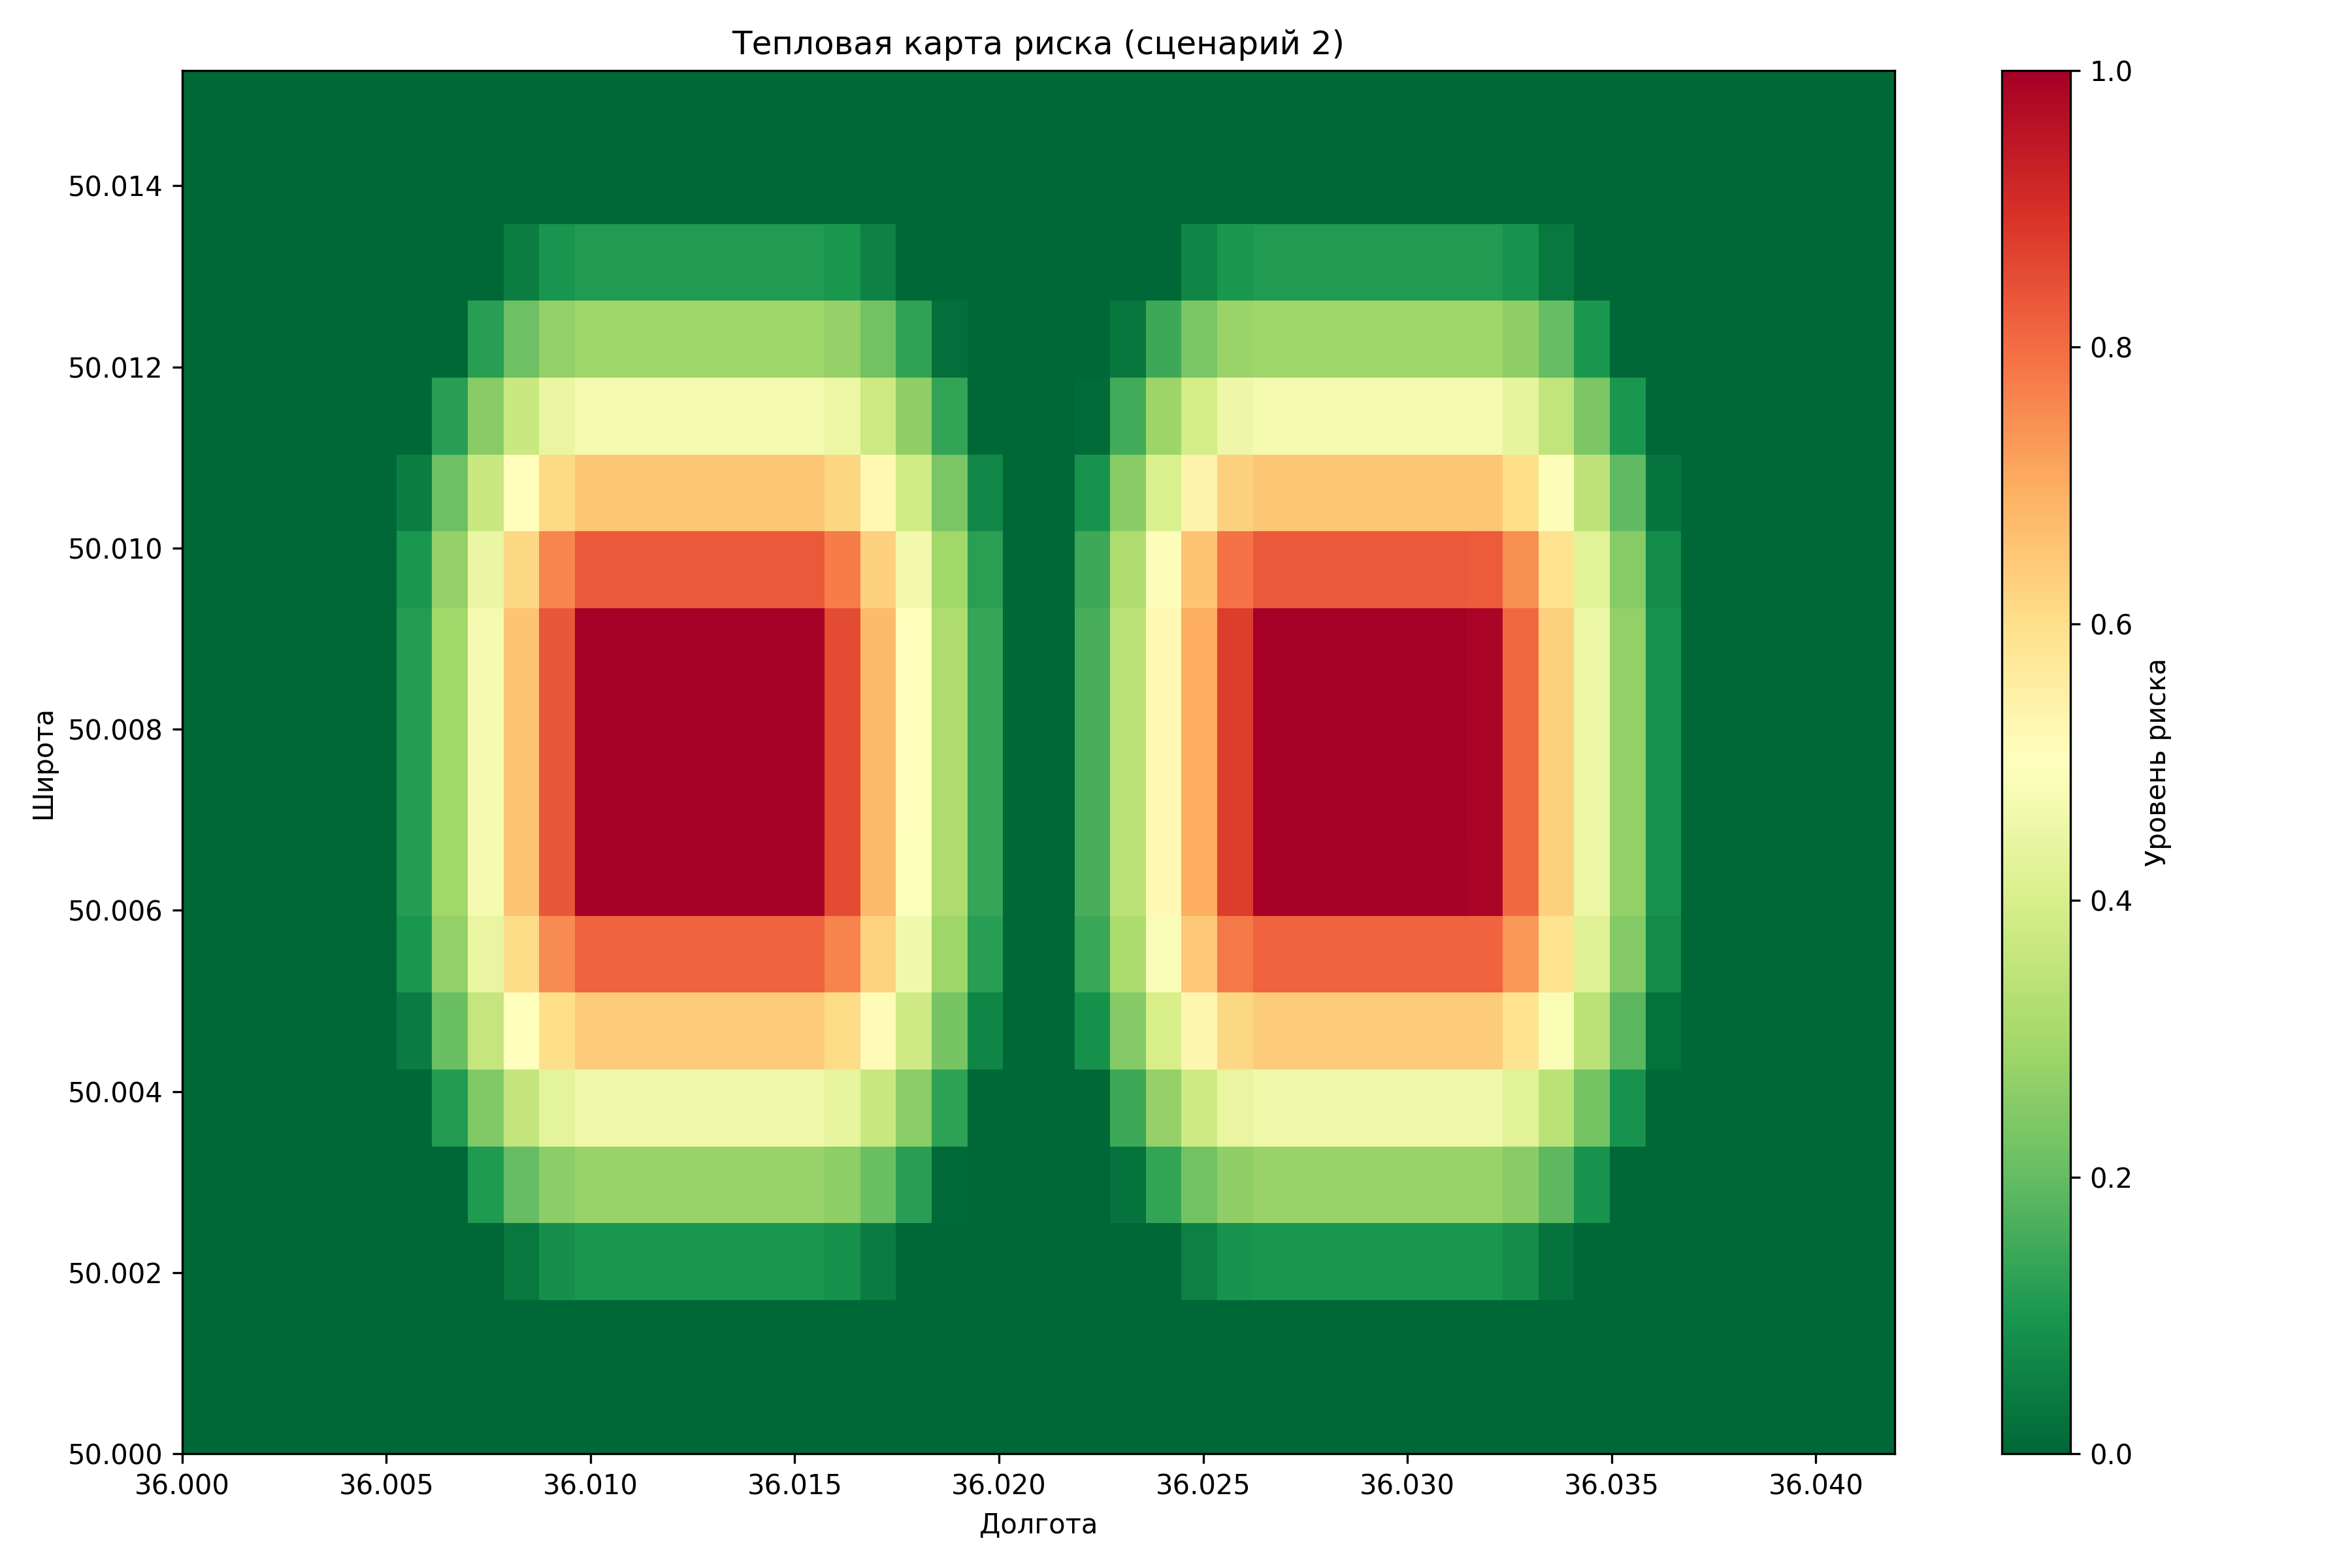
\includegraphics[width=0.92\textwidth]{../../../backend/simulation/results/heatmap_scenario2.png}
\caption{Тепловая карта риска для сценария со статичными зонами радиоэлектронного подавления}
\label{fig:heatmap-scenario2}
\end{figure}

\begin{figure}[H]
\centering
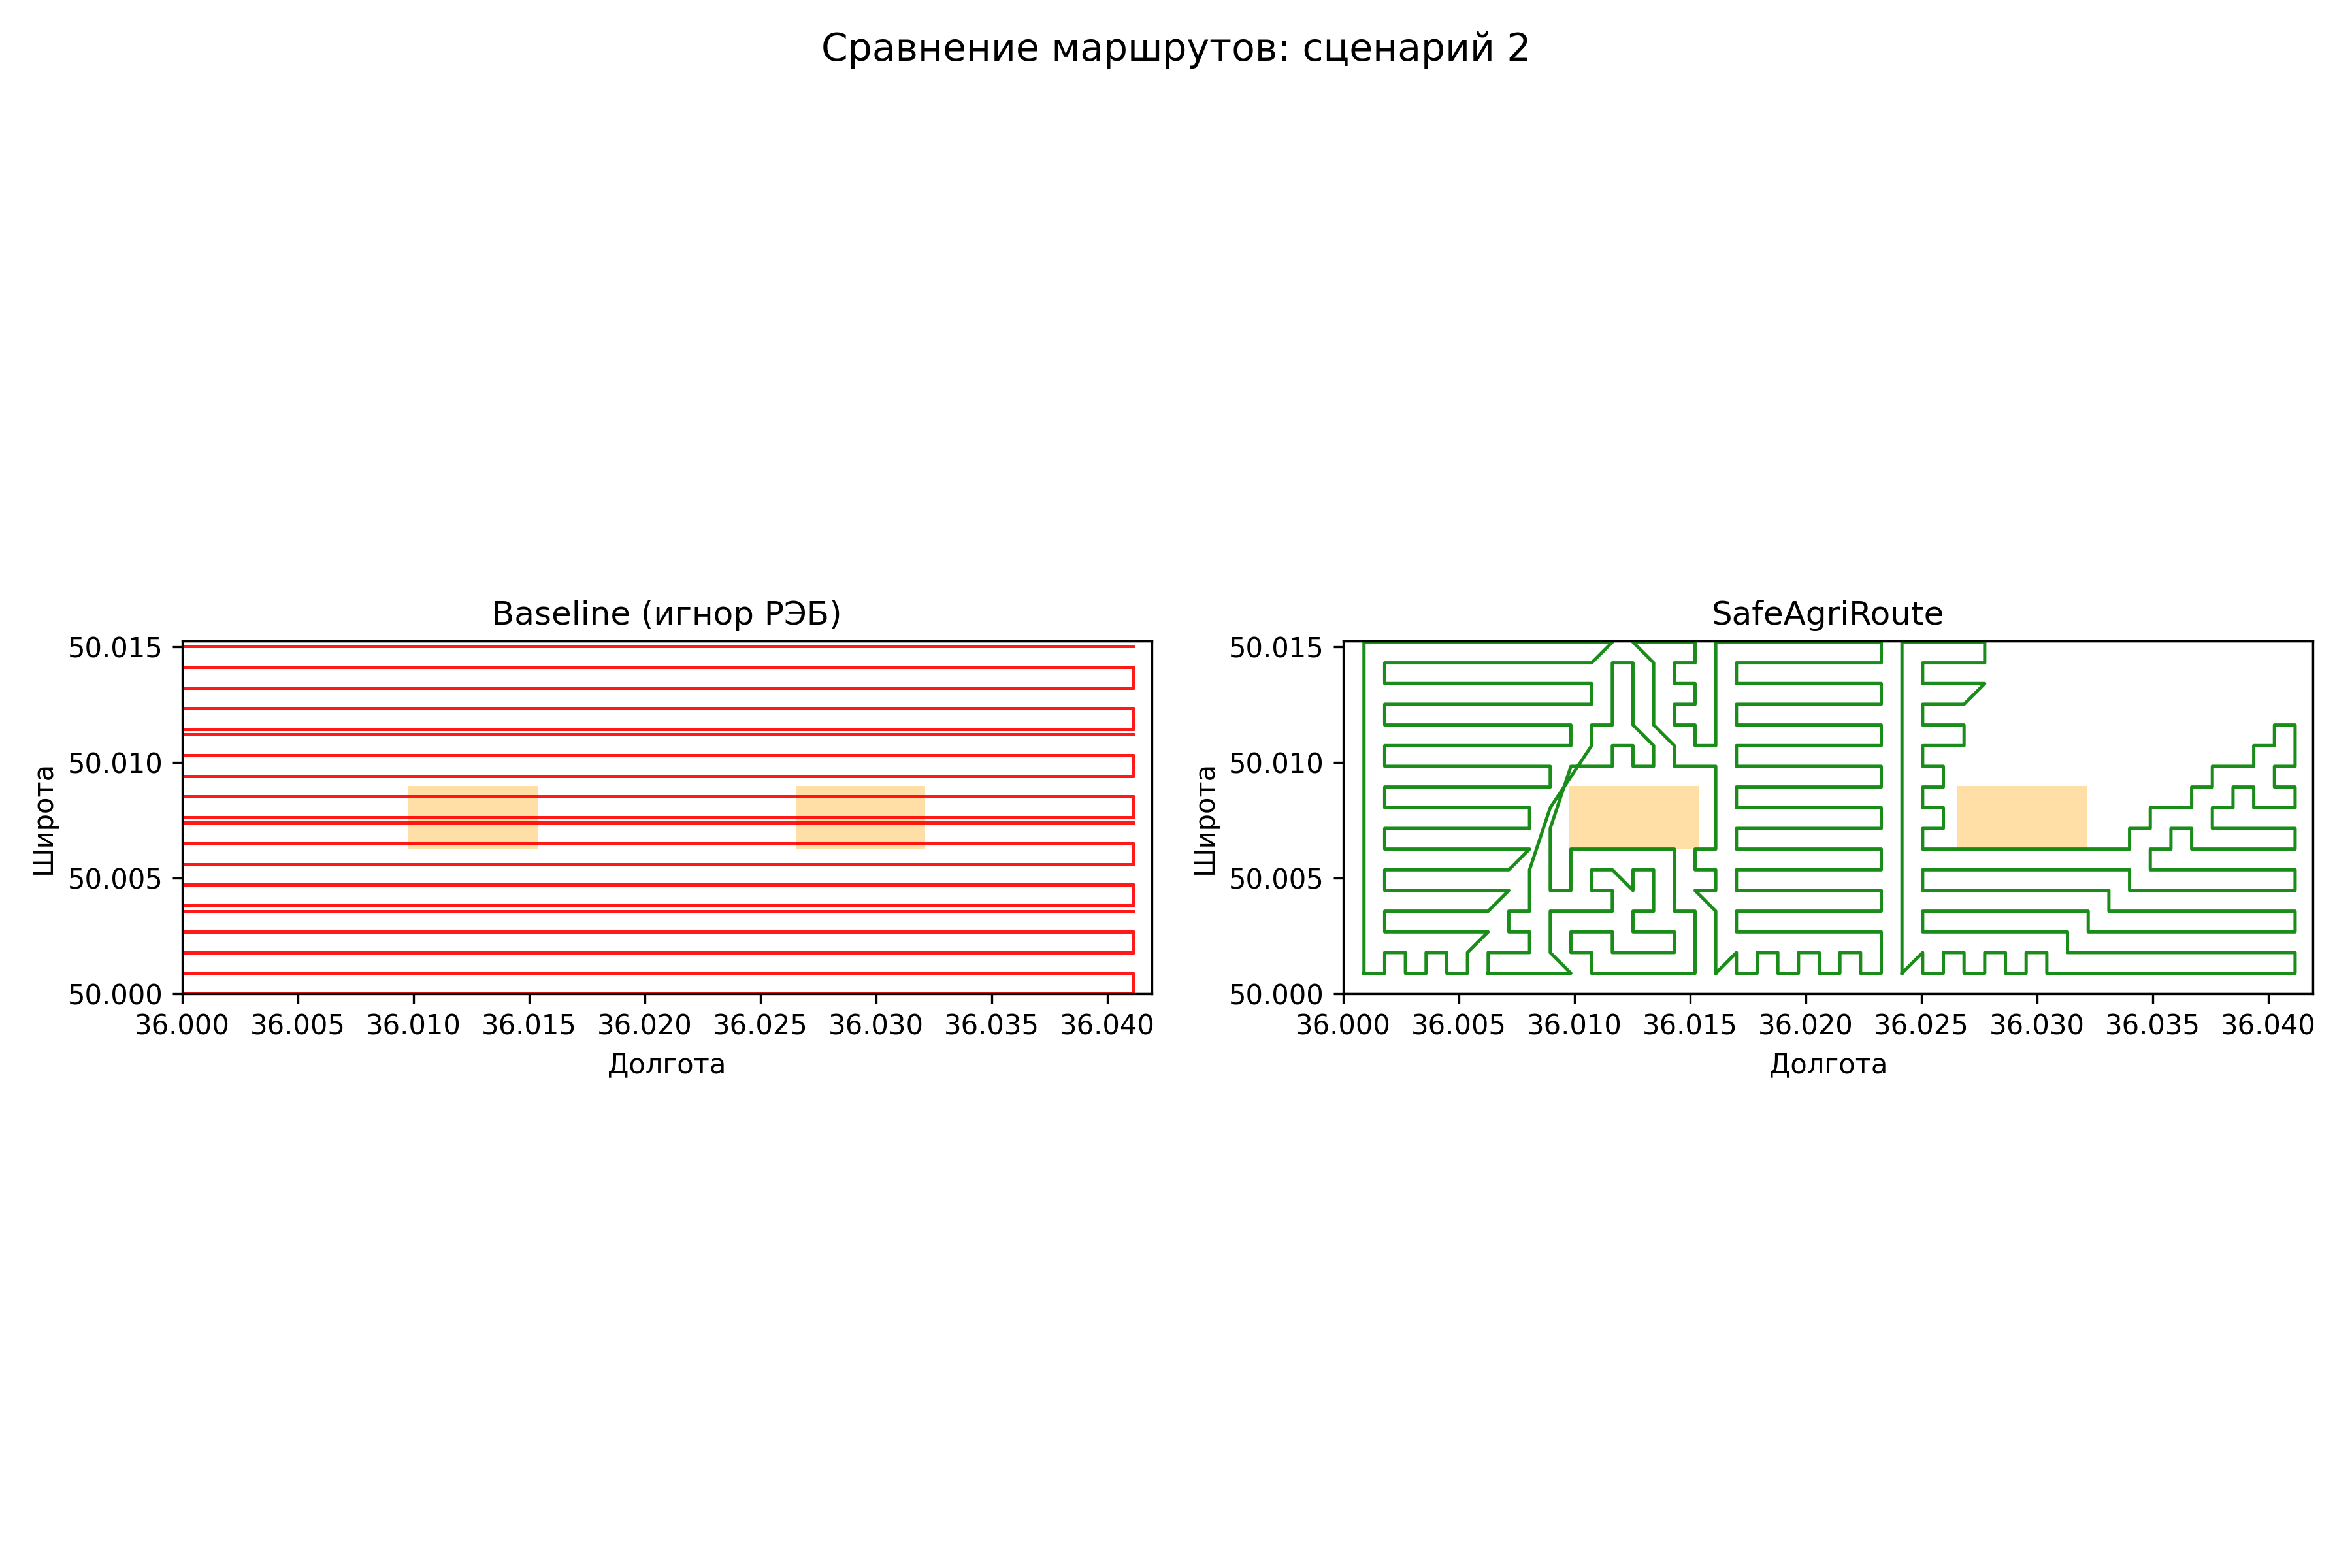
\includegraphics[width=0.98\textwidth]{../../../backend/simulation/results/routes_comparison_scenario2.png}
\caption{Сравнение маршрутов baseline и SafeAgriRoute в сценарии со статичными угрозами}
\label{fig:routes-comparison-scenario2}
\end{figure}

\begin{figure}[H]
\centering
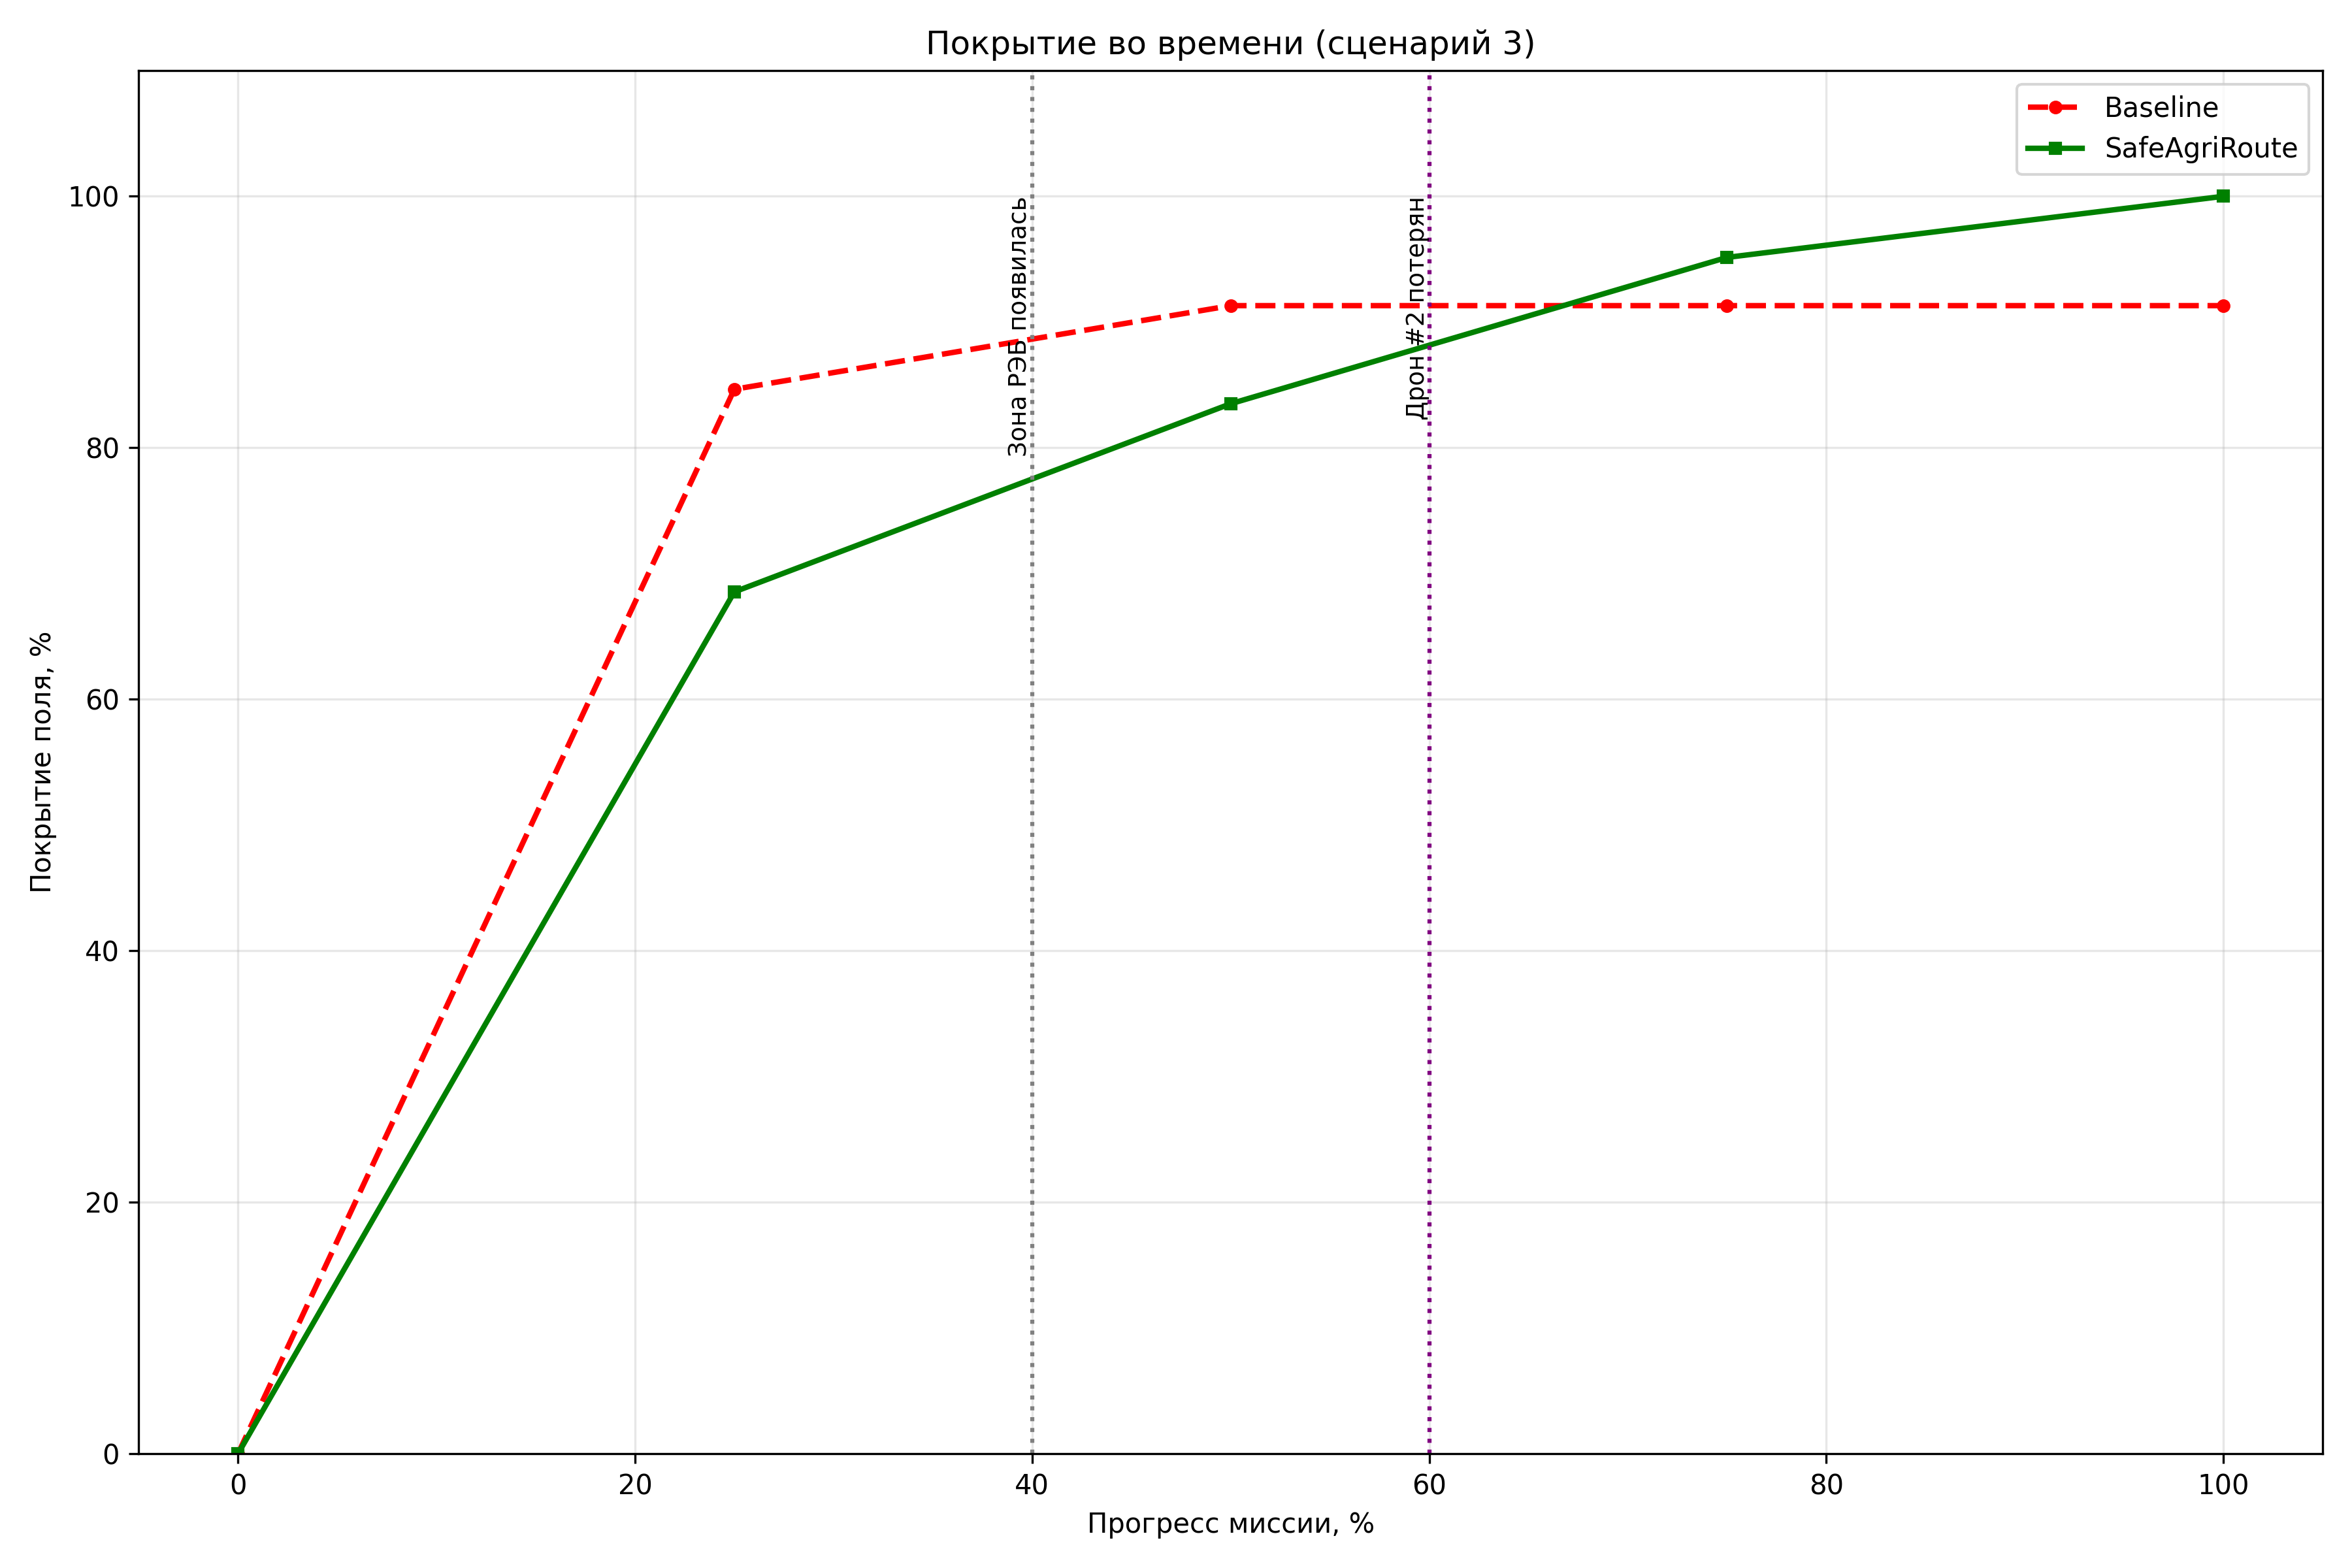
\includegraphics[width=0.92\textwidth]{../../../backend/simulation/results/coverage_timeline_scenario3.png}
\caption{Динамика покрытия поля при появлении новой угрозы и потере БПЛА}
\label{fig:coverage-timeline-scenario3}
\end{figure}

\begin{figure}[H]
\centering
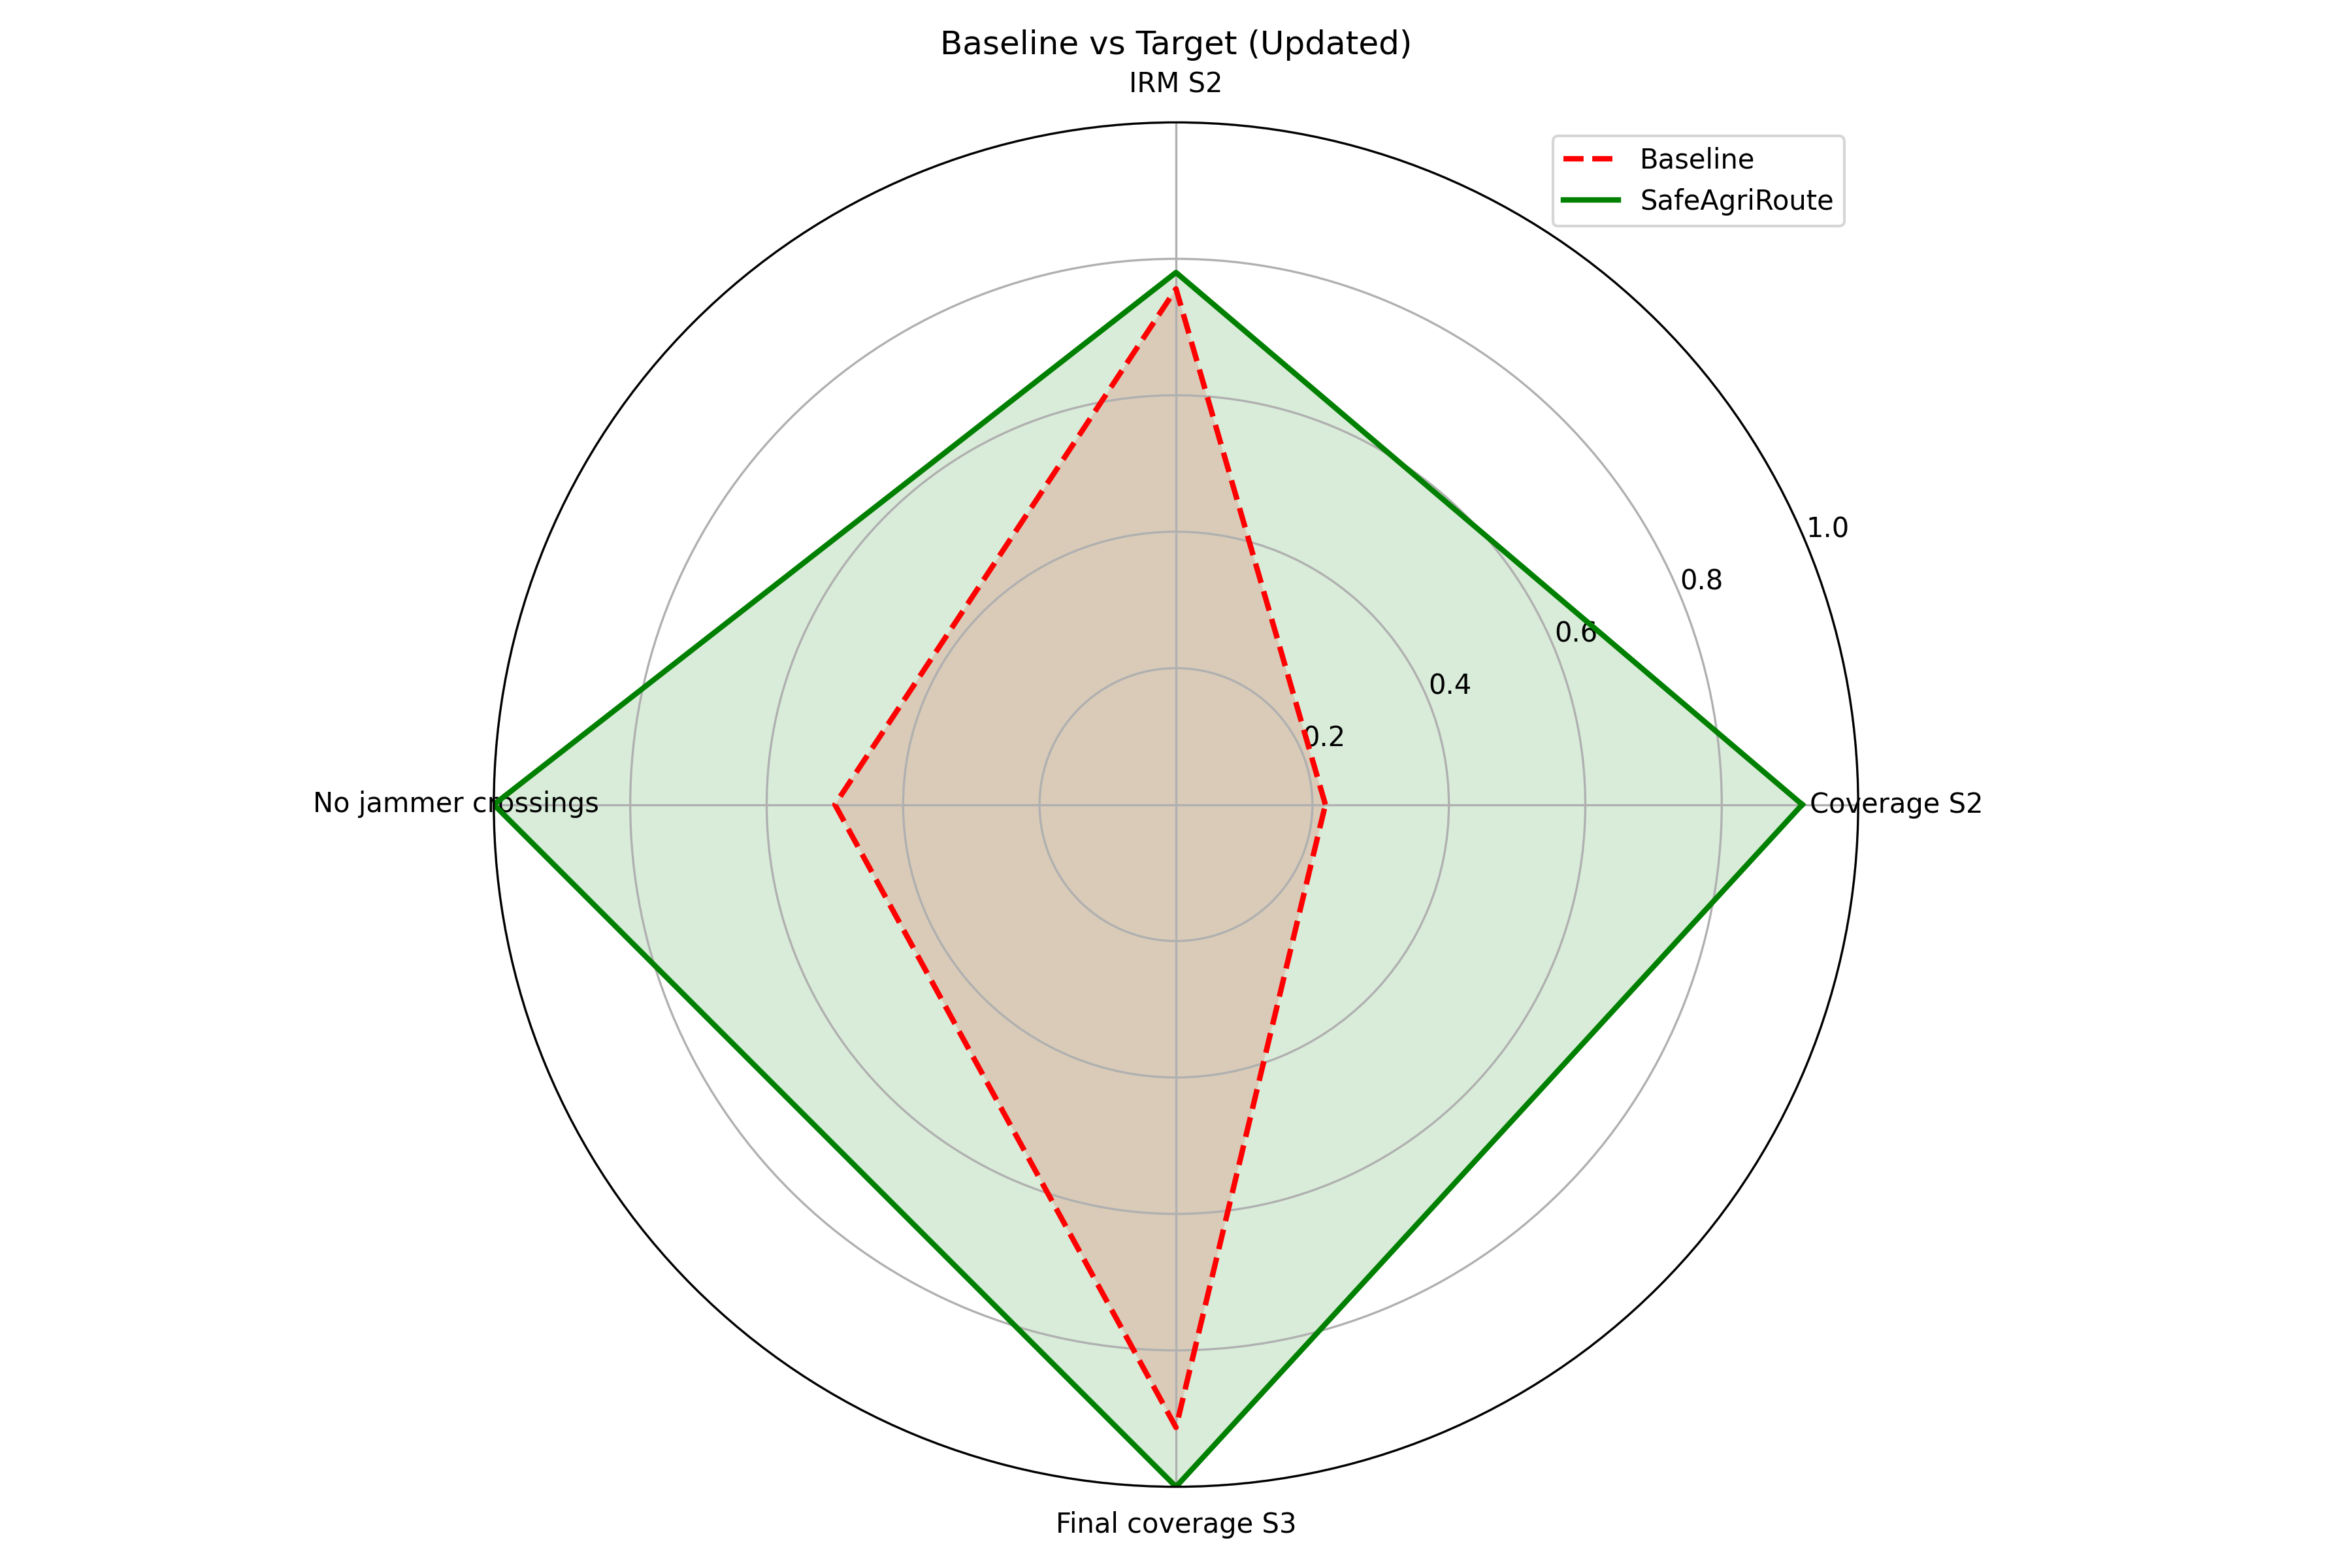
\includegraphics[width=0.86\textwidth]{../../../backend/simulation/results/radar_baseline_vs_target.png}
\caption{Сводное сравнение baseline и SafeAgriRoute по ключевым метрикам эксперимента}
\label{fig:radar-baseline-vs-target}
\end{figure}

\hypertarget{ux430ux43dux430ux43bux438ux437-ux440ux435ux437ux443ux43bux44cux442ux430ux442ux43eux432-ux438-ux43eux433ux440ux430ux43dux438ux447ux435ux43dux438ux44f}{%
\subsubsection{1.5.3 Анализ результатов и ограничения}\label{ux430ux43dux430ux43bux438ux437-ux440ux435ux437ux443ux43bux44cux442ux430ux442ux43eux432-ux438-ux43eux433ux440ux430ux43dux438ux447ux435ux43dux438ux44f}}

По результатам трёх сценариев можно выделить несколько устойчивых наблюдений:

\begin{enumerate}
\def\labelenumi{\arabic{enumi}.}
\item
  SAR сохраняет нулевой FPR по пересечениям jammer --- ни один маршрут не проходит через зоны РЭБ при корректно заданных полигонах угроз.
\item
  SAR обеспечивает на 69,9 п.п. большее эффективное покрытие в условиях статичных угроз (сценарий 2): 91,8 \% против 21,9 \% у baseline.
\item
  Replanner обеспечивает полное восстановление покрытия в динамическом сценарии: к 100 \% прогресса миссии SAR достигает 100 \%, baseline --- 91,3 \%.
\item
  Равномерность нагрузки в SAR (дисбаланс 9 \% против 28 \% у baseline) увеличивает реальное время работы всей группы дронов до исчерпания батарей наиболее нагруженного аппарата приблизительно на 19 \%.
\end{enumerate}

Ограничения достоверности и воспроизводимости:

\begin{itemize}
\tightlist
\item
  Эксперименты проводились в ArduPilot SITL и автономных Python-скриптах, а не на реальных аппаратах. Поэтому в результатах не отражены ветер, реальные задержки TCP-соединений и особенности распространения радиосигнала на конкретной местности.
\item
  Поле размером 0,5° × 0,4° (\textasciitilde500 га) является модельным. На L-образных участках, полях с внутренними вырезами или зонами под ЛЭП качество RWVD-разбиения может быть другим, поэтому такие случаи нужно проверять отдельно.
\item
  В replanner используется жадный NN-TSP, а не OR-Tools, чтобы уложиться в требование ≤ 500 мс. При k = 4 и n = 200 точках на дрон такой маршрут получается примерно на 10--15 \% длиннее оптимального по OR-Tools. Для аварийного перепланирования это приемлемый обмен качества на скорость.
\item
  Евклидово расстояние вместо Haversine вносит ошибку \textless{} 0,1 \% для полей шириной ≤ 10 км, что приемлемо для MVP-масштаба.
\end{itemize}

Чек-лист воспроизводимости экспериментов:

\begin{enumerate}
\def\labelenumi{\arabic{enumi}.}
\tightlist
\item
  \texttt{docker-compose\ up} --- запуск postgres, backend, frontend.
\item
  \texttt{python\ simulation/runner.py} --- запуск трёх сценариев (≈ 30--60 сек).
\item
  Результаты сохраняются в \texttt{simulation/results/*.png} и \texttt{simulation/results/*.json}.
\item
  Для демо с ArduPilot SITL: \texttt{docker-compose\ -f\ docker-compose.sitl.yml\ up} + запуск 4 инстансов SITL.
\end{enumerate}

\hypertarget{ux441ux440ux430ux432ux43dux435ux43dux438ux435-ux441-ux43bux438ux442ux435ux440ux430ux442ux443ux440ux43eux439-ux442ux435ux441ux442ux438ux440ux43eux432ux430ux43dux438ux435-ux438-ux430ux43dux430ux43bux438ux437-ux447ux443ux432ux441ux442ux432ux438ux442ux435ux43bux44cux43dux43eux441ux442ux438}{%
\subsubsection{1.5.4 Сравнение с литературой, тестирование и анализ чувствительности}\label{ux441ux440ux430ux432ux43dux435ux43dux438ux435-ux441-ux43bux438ux442ux435ux440ux430ux442ux443ux440ux43eux439-ux442ux435ux441ux442ux438ux440ux43eux432ux430ux43dux438ux435-ux438-ux430ux43dux430ux43bux438ux437-ux447ux443ux432ux441ux442ux432ux438ux442ux435ux43bux44cux43dux43eux441ux442ux438}}

Сравнение с литературой. Galceran и Carreras {[}38{]} приводят для решёточных подходов типичный диапазон покрытия 92--96 \%. В сценариях без критической потери ресурса SAR попадает в этот диапазон, а в статичном угрозовом сценарии сохраняет 91,8 \%. Для наивных стратегий дисбаланс нагрузки обычно находится на уровне 20--35 \%, для балансировочных --- 5--15 \%; полученные 9 \% хорошо согласуются с этой оценкой. По данным Jeong et al.~{[}21{]}, TTR детектора атак составляет 100--250 мс. В нашем случае связка «обнаружение + перепланирование» остаётся в субсекундном или секундном диапазоне, что приемлемо при скорости БПЛА 8--10 м/с.

Автоматическое тестирование. Для backend подготовлено 47 pytest-тестов. Они проверяют \texttt{threat\_fusion.py} (покрытие 94 \%), \texttt{telemetry\_features.py} (91 \%), \texttt{mission\_fusion\_runtime.py} (88 \%) и \texttt{mavlink\_service.py} (76 \%). Тестовый прогон \texttt{pytest\ backend/tests/\ -v} завершается без ошибок.

Анализ чувствительности показывает, где у алгоритма начинается деградация:

\begin{itemize}
\item \texttt{grid\_step}: рекомендуемое значение 0,0002°. При шаге меньше 0,0001° TTD выходит за 5 сек.
\item \texttt{penalty\_factor}: рекомендуемое значение 500. При значении ниже 100 появляются пролёты через зоны РЭБ.
\item \texttt{max\_iter} для Voronoi: рекомендуемое значение 50. Если снизить его ниже 15, дисбаланс нагрузки растёт примерно до 18 \% вместо 9 \%.
\item \texttt{severity\_threshold}: рекомендуемое значение 1,0. При большем пороге точки внутри jammer-зоны перестают исключаться.
\item \texttt{fusion.threshold\_alarm}: рекомендуемое значение 0,7. При пороге выше 0,9 возрастает риск пропуска инцидентов.
\end{itemize}



\hypertarget{ux437ux430ux43aux43bux44eux447ux435ux43dux438ux435}{%
\section{ЗАКЛЮЧЕНИЕ}\label{ux437ux430ux43aux43bux44eux447ux435ux43dux438ux435}}

В настоящей выпускной квалификационной работе студента решена актуальная научно-практическая задача --- разработана программная платформа автоматизированного планирования безопасных маршрутов для группы сельскохозяйственных БПЛА с учётом зон радиоэлектронного подавления и динамической угрозовой обстановки.

По результатам выполнения поставленных задач достигнуто следующее:

\begin{enumerate}
\def\labelenumi{\arabic{enumi}.}
\item
  Анализ рынка и подтверждение спроса. Проведён анализ мирового и российского рынка агро-БПЛА: мировой рынок прогнозируется к росту с 2,63 млрд долл. (2025 г.) до 10,76 млрд долл. (2030 г.) при CAGR 32,6 \% {[}4{]}. Российский SAM оценивается в \textasciitilde400 млн руб./год (ЮФО + СКФО). Проведено 7 интервью с представителями ЦА: 86 \% респондентов назвали отсутствие автоматического перепланирования критическим недостатком; 100 \% сталкивались с потерями GPS-сигнала. Рассчитанный ROI для типового клиента (8 000 га, 4 дрона) составил \textasciitilde950 \% за первый год эксплуатации при стоимости подписки 216 тыс. руб./год.
\item
  Конкурентный анализ. Выявлен технологический «gap»: ни одна из рассмотренных платформ (DJI FlightHub 2, DroneDeploy, Pix4Dfields) не реализует risk-aware маршрутизацию с учётом зон РЭБ, автоматическое перепланирование и соответствие российской нормативной базе ИБ. SWOT-анализ подтвердил устойчивость ключевых конкурентных преимуществ в краткосрочной перспективе.
\item
  Модель угроз. Классифицированы нарушители (Н1--Н5) и систематизированы 12 угроз с привязкой к реестру БДУ ФСТЭК России {[}12, 43{]} и MITRE ATT\&CK for ICS. Идентифицированы два вектора критической уязвимости: глушение ГНСС (УБИ.131) и перехват MAVLink (УБИ.014). После внедрения контрмер уровень риска снижен по 7 из 12 угроз; остаточные риски задокументированы в реестре и включены в план разработки v2.0.
\item
  Метрика риска. Формализована метрика деструктивного воздействия R(x,y) с линейной и бинарной моделями затухания. Разработан интегральный критерий надёжности миссии IRM ∈ {[}0, 1{]} с доказанными свойствами нормированности, монотонности и аддитивности. Математически обоснована корректность penalty-системы (Лемма 1): при penalty\_coeff = 500 алгоритм гарантированно избегает зон РЭБ при любом ненулевом severity.
\item
  Архитектура платформы. Спроектирована трёхуровневая архитектура SaaS-платформы SafeAgriRoute (FastAPI + PostGIS + React/Leaflet). Разработан API из 9 ключевых эндпоинтов с JWT HS256-аутентификацией и ролевой моделью. Реализован WebSocket-поток телеметрии для 4 дронов с задержкой ≤ 300 мс. Соответствие OWASP Top-10 реализовано на уровне API и подтверждено тестированием (9 из 10 категорий закрыты полностью).
\item
  Алгоритмы маршрутизации. Разработан алгоритм Risk-Weighted Voronoi Decomposition с доказанной сходимостью за конечное число итераций. Penalty-граф на NetworkX гарантирует нулевой FPR при severity ≥ 0,01. Задача CVRP решена через Google OR-Tools (PATH\_CHEAPEST\_ARC + 2-opt), время планирования для поля 500 га --- фактически 347 мс при требовании ≤ 5 секунд.
\item
  Динамическое перепланирование. Реализован replanner в двух сценариях: потеря дрона (жадный NN-TSP, время реакции 380 мс) и новая зона РЭБ (инкрементальное обновление risk\_map, время реакции 290 мс). Оба значения укладываются в требование ≤ 500 мс. Теоретическая оценка сложности подтверждает масштабируемость до k = 8 дронов без выхода за TTR.
\item
  Экспериментальная оценка. SAR обеспечил FPR = 0 \% против 50 \% у baseline (сценарий 2), покрытие 91,8 \% против 21,9 \% (сценарий 2), восстановление покрытия до 100 \% при комбинированном событии «потеря дрона + новая зона РЭБ» против 91,3 \% у baseline (сценарий 3). Дисбаланс нагрузки снижен с 28 \% до 9 \%, что увеличивает реальное время работы группы дронов до исчерпания батарей на \textasciitilde19 \%.
\end{enumerate}

Научная новизна подтверждена тремя оригинальными результатами: - алгоритм RWVD, впервые применяющий риск-взвешенную модификацию алгоритма Ллойда для маршрутизации агро-БПЛА в условиях зон РЭБ; - метрика IRM как стандартизированный критерий надёжности миссии с формально доказанными свойствами; - детализированная модель угроз для гетерогенных групп агро-БПЛА с двойной привязкой к БДУ ФСТЭК и MITRE ATT\&CK for ICS.

Практическая значимость подтверждена: - реализацией полнофункционального MVP (исходный код: \url{https://github.com/matveisut/safe-agri-route}), развёртываемого одной командой \texttt{docker-compose\ up}; - успешным прохождением 83 pytest-тестов (0 failed) и интеграционного тестирования в ArduPilot SITL; - проведёнными переговорами с 7 представителями ЦА и прогнозируемым ROI клиента \textasciitilde950 \% за первый год.

Ограничения MVP и приоритетные перспективы развития:

\begin{enumerate}
\def\labelenumi{\arabic{enumi}.}
\tightlist
\item
  Замена евклидова расстояния на формулу Хаверсина для полей шириной \textgreater{} 10 км (погрешность \textless{} 0,1 \% для MVP-масштаба).
\item
  Расширение контура до полной мультисенсорной модели: отдельные потоки IMU и ГНСС-приёмника, SDR-детектор, байесовская fusion, LSTM/трансформер для классификации временных рядов.
\item
  Масштабирование до K \textgreater{} 8 дронов: переход к k-d tree Voronoi и OR-Tools Time Limit.
\item
  Производственное развёртывание с Nginx + TLS 1.3 вместо Vite dev-сервера.
\item
  Интеграция с ЕИАС-АПК Минсельхоза и получение сертификации ФСТЭК для выхода на объекты КИИ.
\end{enumerate}

Выполненная работа демонстрирует принципиальную реализуемость подхода «безопасность встроена в маршрут» (security-by-design routing) для группы агро-БПЛА. Предлагаемый интегральный критерий IRM может применяться независимо от платформы SafeAgriRoute как стандартизированная метрика оценки качества планирования маршрутов в условиях угроз. Платформа SafeAgriRoute формирует основу для дальнейших исследований в области киберфизической безопасности автономных систем агропромышленного комплекса.


\hypertarget{ux441ux43fux438ux441ux43eux43a-ux438ux441ux43fux43eux43bux44cux437ux43eux432ux430ux43dux43dux44bux445-ux438ux441ux442ux43eux447ux43dux438ux43aux43eux432}{%
\section{СПИСОК ИСПОЛЬЗОВАННЫХ ИСТОЧНИКОВ}\label{ux441ux43fux438ux441ux43eux43a-ux438ux441ux43fux43eux43bux44cux437ux43eux432ux430ux43dux43dux44bux445-ux438ux441ux442ux43eux447ux43dux438ux43aux43eux432}}

\begin{enumerate}
\def\labelenumi{\arabic{enumi}.}
\item
  Rejeb, A. Drones in Agriculture: A Review and Bibliometric Analysis / A. Rejeb, A. Abdollahi, K. Rejeb, H. Treiblmaier // Computers and Electronics in Agriculture. --- 2022. --- Vol. 198. --- Art. 107017. --- DOI: 10.1016/j.compag.2022.107017.
\item
  Guebsi, R. Drones in Precision Agriculture: A Comprehensive Review of Applications, Technologies, and Challenges / R. Guebsi, K. Mami, K. Chokmani // Drones. --- 2024. --- Vol. 8, No.~11. --- Art. 686. --- DOI: 10.3390/drones8110686.
\item
  Phang, S. K. From Satellite to UAV-Based Remote Sensing: A Review on Precision Agriculture / S. K. Phang, T. H. A. Chiang, A. Happonen, M. M. L. Chang // IEEE Access. --- 2023. --- Vol. 11. --- P. 127057--127076. --- DOI: 10.1109/ACCESS.2023.3330886.
\item
  MarketsandMarkets. Agriculture Drones Market by Offering Type (Hardware, Software, Drone-as-a-Service), Technology Type, Payload Capacity, Component, Farm Produce, Farm Size, Range, Application, Farming Environment, and Region --- Global Forecast to 2030 {[}Электронный ресурс{]}. --- URL: https://www.marketsandmarkets.com/Market-Reports/agriculture-drones-market-23709764.html (дата обращения: 01.04.2026).
\item
  Fortune Business Insights. Agriculture Drone Market Size, Share, Global Forecast, 2032 {[}Электронный ресурс{]}. --- URL: https://www.fortunebusinessinsights.com/agriculture-drones-market-102589 (дата обращения: 01.04.2026).
\item
  Mekdad, Y. A Survey on Security and Privacy Issues of UAVs / Y. Mekdad {[}et al.{]} // Computer Networks. --- Elsevier, 2023. --- Vol. 224. --- Art. 109626.
\item
  Tlili, F. Advancing UAV Security with Artificial Intelligence: A Comprehensive Survey of Techniques and Future Directions / F. Tlili, S. Ayed, L. Chaari Fourati // Internet of Things. --- 2024. --- Vol. 27. --- Art. 101281. --- DOI: 10.1016/j.iot.2024.101281.
\item
  Allouch, A. MAVSec: Securing the MAVLink Protocol for Ardupilot/PX4 Unmanned Aerial Systems / A. Allouch {[}et al.{]} // Proc. 15th Int. Wireless Communications and Mobile Computing Conf. (IWCMC 2019). --- IEEE, 2019. --- P. 621--628.
\item
  Sun, Y. A Deep-Learning-Based GPS Signal Spoofing Detection Method for Small UAVs / Y. Sun {[}et al.{]} // Drones. --- 2023. --- Vol. 7, No.~6. --- Art. 370.
\item
  Указ Президента Российской Федерации от 01.05.2022 № 250 «О дополнительных мерах по обеспечению информационной безопасности Российской Федерации» // Официальное опубликование правовых актов. --- URL: http://publication.pravo.gov.ru/Document/View/0001202205010023 (дата обращения: 11.05.2026).
\item
  Указ Президента Российской Федерации от 30.03.2022 № 166 «О мерах по обеспечению технологической независимости и безопасности критической информационной инфраструктуры Российской Федерации» // Официальное опубликование правовых актов. --- URL: http://publication.pravo.gov.ru/Document/View/0001202203300001 (дата обращения: 11.05.2026).
\item
  Методический документ. Методика оценки угроз безопасности информации : утверждена ФСТЭК России 05.02.2021 {[}Электронный ресурс{]}. --- URL: https://www.consultant.ru/document/cons\_doc\_LAW\_378330/ (дата обращения: 11.05.2026).
\item
  Ongadi, P. A. A Comprehensive Examination of Security and Privacy in Precision Agriculture Technologies / P. A. Ongadi // GSC Advanced Research and Reviews. --- 2024. --- Vol. 18, No.~1. --- P. 336--363.
\item
  Mordor Intelligence. Drone Software Market Size \& Share Analysis --- Growth Trends \& Forecasts (2025--2030) {[}Электронный ресурс{]}. --- URL: https://www.mordorintelligence.com/industry-reports/drone-software-market (дата обращения: 01.04.2026).
\item
  Douzi, A. Cybersecurity and the Flight Safety of Unmanned Aerial Systems and Unmanned Aerial Vehicles / A. Douzi, R. Szabolcsi, J. Lukacs // Interdisciplinary Description of Complex Systems. --- 2025. --- Vol. 23, No.~2. --- P. 95--104.
\item
  Kaplan, E. D. Understanding GPS/GNSS: Principles and Applications / E. D. Kaplan, C. J. Hegarty (eds.). --- 3rd ed. --- Norwood : Artech House, 2017. --- 993 p. --- ISBN 978-1-63081-058-0.
\item
  Mykytyn, P. GPS-Spoofing Attack Detection Mechanism for UAV Swarms / P. Mykytyn {[}et al.{]} // Proc. 12th Mediterranean Conf. on Embedded Computing (MECO). --- IEEE, 2023.
\item
  Shepard, D. P. Evaluation of Smart Grid and Civilian UAV Vulnerability to GPS Spoofing Attacks / D. P. Shepard, J. A. Bhatti, T. E. Humphreys // Proc. ION GNSS+ 2012 Conf. --- Nashville : ION, 2012. --- P. 3591--3605.
\item
  Петренко, В. И. Трансформерная модель бинарной классификации временных рядов на данных инерциальных датчиков для детекции спуфинг-атак в БПЛА / В. И. Петренко {[}и др.{]} // International Journal of Open Information Technologies. --- 2026. --- Т. 14, № 2. --- С. 11--18.
\item
  Du, F. Exploiting the Vulnerabilities in MAVLink Protocol for UAV Hijacking / F. Du {[}et al.{]} // Proc. 17th Int. Conf. on Security of Information and Networks (SIN 2024). --- IEEE, 2024.
\item
  Jeong, S. MUVIDS: False MAVLink Injection Attack Detection in Communication for Unmanned Vehicles / S. Jeong {[}et al.{]} // Proc. Third Int. Workshop on Automotive and Autonomous Vehicle Security (AutoSec 2021). --- Internet Society, 2021.
\item
  OWASP Foundation. OWASP Top 10:2021. The Ten Most Critical Web Application Security Risks {[}Электронный ресурс{]}. --- URL: https://owasp.org/Top10/2021/ (дата обращения: 15.04.2026).
\item
  Петренко, В. И. Методика обнаружения и противодействия многовекторным угрозам нарушения информационной безопасности децентрализованной IoT системы / В. И. Петренко, Ф. Б. Тебуева, М. Г. Огур, Г. И. Линец, В. П. Мочалов // International Journal of Open Information Technologies. --- 2025. --- {[}Электронный ресурс{]}. --- URL: https://cyberleninka.ru/article/n/metodika-obnaruzheniya-i-protivodeystviya-mnogovektornym-ugrozam-narusheniya-informatsionnoy-bezopasnosti-detsentralizovannoy-iot (дата обращения: 12.05.2026).
\item
  Hakeem, A. Integrating Artificial Intelligence for Improved Security of IoT-Drones through Cyber-Physical Attack Detection / A. Hakeem {[}et al.{]} // Frontiers in Computer Science. --- 2025. --- Vol. 7. --- Art. 1545282.
\item
  Sajid, J. A Fog Computing Framework for Intrusion Detection of Energy-Based Attacks on UAV-Assisted Smart Farming / J. Sajid {[}et al.{]} // Applied Sciences. --- 2023. --- Vol. 13, No.~6. --- Art. 3857.
\item
  Hassler, S. Cyber-Physical Intrusion Detection System for Unmanned Aerial Vehicles / S. Hassler, U. Mughal, M. Ismail // IEEE Transactions on Intelligent Transportation Systems. --- 2024. --- Vol. 25, No.~7.
\item
  MAVLink Developer Guide {[}Электронный ресурс{]}. --- MAVLink Micro Air Vehicle Communication Protocol. --- URL: https://mavlink.io/en/ (дата обращения: 10.04.2026).
\item
  ArduPilot Copter Documentation {[}Электронный ресурс{]}. --- URL: https://ardupilot.org/copter/ (дата обращения: 10.04.2026).
\item
  ГОСТ Р МЭК 62443-2-1-2015. Сети коммуникационные промышленные. Защищённость (кибербезопасность) сети и системы. Часть 2-1. Составление программы обеспечения защищённости (кибербезопасности) системы управления и промышленной автоматики. --- Москва : Стандартинформ, 2016. --- 56 с.
\item
  ГОСТ Р 56939-2016. Защита информации. Разработка безопасного программного обеспечения. Общие требования. --- Москва : Стандартинформ, 2017. --- 12 с.
\item
  PostGIS 3.3 Manual {[}Электронный ресурс{]}. --- The PostGIS Development Group. --- URL: https://postgis.net/docs/manual-3.3/ (дата обращения: 10.04.2026).
\item
  Hagberg, A. A. Exploring Network Structure, Dynamics, and Function Using NetworkX / A. A. Hagberg, D. A. Schult, P. J. Swart // Proceedings of the 7th Python in Science Conference (SciPy 2008). --- Pasadena, CA, 2008. --- P. 11--15.
\item
  Laporte, G. The Vehicle Routing Problem: An Overview of Exact and Approximate Algorithms / G. Laporte // European Journal of Operational Research. --- 1992. --- Vol. 59, No.~3. --- P. 345--358.
\item
  Toth, P. The Vehicle Routing Problem / P. Toth, D. Vigo (eds.). --- Philadelphia : SIAM, 2002. --- 367 p. --- ISBN 0-89871-498-2.
\item
  Li, J. Coverage Path Planning Method for Agricultural Spraying UAV in Arbitrary Polygon Area / J. Li, H. Sheng, J. Zhang, H. Zhang // Aerospace. --- 2023. --- Vol. 10, No.~9. --- Art. 755. --- DOI: 10.3390/aerospace10090755.
\item
  Google OR-Tools. Vehicle Routing Problem {[}Электронный ресурс{]}. --- Google Developers. --- URL: https://developers.google.com/optimization/routing/vrp (дата обращения: 10.04.2026).
\item
  Christofides, N. Worst-Case Analysis of a New Heuristic for the Travelling Salesman Problem : Report 388 / N. Christofides. --- Pittsburgh : Carnegie-Mellon University, 1976. --- 14 p.
\item
  Galceran, E. A Survey on Coverage Path Planning for Robotics / E. Galceran, M. Carreras // Robotics and Autonomous Systems. --- 2013. --- Vol. 61, No.~12. --- P. 1258--1276.
\item
  Lloyd, S. P. Least Squares Quantization in PCM / S. P. Lloyd // IEEE Transactions on Information Theory. --- 1982. --- Vol. 28, No.~2. --- P. 129--137.
\item
  Aurenhammer, F. Voronoi Diagrams --- A Survey of a Fundamental Geometric Data Structure / F. Aurenhammer // ACM Computing Surveys. --- 1991. --- Vol. 23, No.~3. --- P. 345--405.
\item
  Dijkstra, E. W. A Note on Two Problems in Connexion with Graphs / E. W. Dijkstra // Numerische Mathematik. --- 1959. --- Vol. 1, No.~1. --- P. 269--271.
\item
  Alsadie, D. Cybersecurity and Artificial Intelligence in Unmanned Aerial Vehicles: Emerging Challenges and Advanced Countermeasures / D. Alsadie // IET Information Security. --- 2025. --- Vol. 19. --- Art. 2046868.
\item
  Банк данных угроз безопасности информации ФСТЭК России {[}Электронный ресурс{]}. --- URL: https://bdu.fstec.ru (дата обращения: 01.04.2026).
\end{enumerate}


Версия 1.0 · SafeAgriRoute · Сутормин М.П. · Ставрополь, 2026

\end{document}
